\documentclass[a4paper]{article}

\usepackage[english]{babel}
\usepackage[utf8]{inputenc}
\usepackage{algorithm}
\usepackage{algorithmic}
\usepackage{fullpage}
\usepackage{amsmath}
\usepackage{graphicx}
\usepackage[colorinlistoftodos]{todonotes}
\usepackage{hyperref}
\usepackage{amssymb}
\usepackage{outline} \usepackage{pmgraph} \usepackage[normalem]{ulem}
\usepackage{graphicx} \usepackage{verbatim}
\usepackage{fourier}
\usepackage[protrusion=true, expansion=true]{microtype}
\usepackage{sectsty}
\usepackage{url, lipsum}
\usepackage{tgbonum}
\usepackage{hyperref}
\usepackage{xcolor}
\usepackage[T1]{fontenc}
\usepackage{fancyhdr}
\usepackage{mathtools}
\usepackage{amsmath}
\usepackage{lastpage}
\usepackage{listings}
\usepackage{graphicx, wrapfig, subcaption, setspace, booktabs}
% \usepackage{minted} % need `-shell-escape' argument for local compile



\newcommand{\norm}[1]{\|#1 \|}
\newcommand{\Exs}{\mathbb{E}}
\newcommand{\thetastar}{\theta^*}
\newcommand{\thetainf}{\theta_\infty}
\newcommand{\thetainfpone}{\theta_{\infty + 1}}
\newcommand{\xstar}{X^*}
\newcommand{\xinf}{X_{\infty}}
\newcommand{\xinfPone}{X_{\infty + 1}}
\newcommand{\xinfPtwo}{X_{\infty + 2}}
\newcommand{\constLPH}[1]{L_{PH}^{(#1)}}
\newcommand{\constT}[1]{T_{#1}}
\newcommand{\constTprime}[1]{T_{#1}^{\prime}}
\newcommand{\mwlcomment}[1]{{\color{orange} #1}}
\newcommand*{\htwai}[1]{\textbf{\textcolor{red}{To: #1}}}
\newcommand{\stepsize}{\alpha}

\newcommand{\HRule}[1]{\rule{\linewidth}{#1}}
\onehalfspacing
\setcounter{tocdepth}{5}
\setcounter{secnumdepth}{5}

\begin{document}
	
	\fontfamily{cmr}\selectfont
	\title{ \normalsize \textsc{}
		\\ [2.0cm]
		\HRule{0.5pt} \\
		\LARGE \textbf{\uppercase{Nonlinear Markovian Stochastic Approximation}
			\HRule{2pt} \\ [0.5cm]
			\normalsize \today \vspace*{5\baselineskip}}
	}
	
	\date{}
	
	\author{
		Mohammadhadi Hadavi \\ 
		Prof. Hoi-To Wai - Chinese University of Hong Kong \\
		Prof. Wenlong Mou - University of Toronto}
	
	\maketitle
	\newpage
	%\tableofcontents
	%\newpage
	
	\section{Preliminaries}
	
	\textbf{Notations} The Euclidean norm is denoted by $\norm{.}$. The lowercase letter $c$ and its derivatives $c^{\prime}, c_{0},$ etc. denote universal numerical constants, whose value may change from line to line. As we are primarily interested in dependence of $\stepsize$ and $k$, we adopt the following big-$O$ notation: $\norm{f} = \mathcal{O}\left(h\left(\stepsize, k\right)\right)$ if it holds that $\norm{f} \le s \cdot \norm{h\left(\stepsize, k\right)}$ for some constant $s > 0$.
	
	We use of the following iteration scheme:
	\begin{align*}
		\theta_{t + 1} = \theta_{t} + \stepsize\left(g\left(\theta_{t}, X_{t + 1}\right) + \xi_{t + 1}\left(\theta_{t}\right)\right)
	\end{align*}
	where $g: \mathbb{R}^{d} \times \mathcal{X} \to \mathbb{R}^{d}$ is a deterministic function, $\{\xi_{k}\}_{k \ge 1}$ are $i.i.d$ zero-mean random fields, and $\stepsize > 0$ is a constant stepsize. We shall omit the superscript $^{(\stepsize)}$ in $\theta_{k}$ when the dependence on $\stepsize$ is clear from the context. 
	
	In our settings, $\{X_{n}, n \in \mathbb{N}\}$ is a \textit{state-dependent} (or controlled) Markov chain, \textit{i.e.,} for any bounded measurable function $g: \mathbb{R}^{d} \times \mathcal{X} \to \mathbb{R}^{d}$,
	\begin{align*}
		\Exs\left[g\left(\theta_{n}, X_{n + 1}\right) | \mathcal{F}_{n}\right] = P_{\theta_{n}}g\left(\theta_{n}, X_{n}\right) = \int g\left(\theta_{n}, x\right)P_{\theta}\left(X_{n}, dx\right),
	\end{align*} 
	where $P_{\theta}: \mathcal{X} \times \mathcal{X} \to \mathbb{R}_{+}$ is a Markov kernel such that, for each $\theta \in \Theta$, $P_{\theta}$ has a unique stationary distribution $\pi_{\theta}$. Also, $\mathcal{F}_{n}$ denotes the filtration generated by the random variables $\left(\theta_{0}, \{\xi_{m + 1}\}_{m \leq n - 1}, \{X_{m}\}_{m \leq n}\right)$.
	
	\subsection{Assumptions}
	\textbf{Assumption 1} \textit{
		For each $X \in \mathcal{X}$, the function $g\left(\theta, X\right)$ is three times continuously differentiable in $\theta$ with uniformly bounded first to third derivatives, i.e., $\sup_{\theta \in \mathbb{R}^{d}}\norm{g^{(i)}\left(\theta, X\right)} < \infty$ for $i = 1, 2, 3, X \in \mathcal{X}$. Moreover, there exists a constant $L_{1} > 0$ such that (1) $\norm{g^{(i)}\left(\theta, X\right) - g^{(i)}\left(\theta^{\prime}, X\right)} \le L_{1}$, for all $\theta, \theta^{\prime} \in \mathbb{R}^{d}, i = 0, 1, 2$ and $X \in \mathcal{X}$, and (2) $\norm{g^{(i)}\left(0, X\right)} \le L_{1}$ for all $X \in \mathcal{X}$ and $i = 0, 1, 2$.
	}
	
	Assumption 1 implies that $g\left(\theta, X\right)$ is $L_{1}$-Lipschitz w.r.t $\theta$ uniformly in $X$. The above assumption immediately implies that the growth of $\norm{g}$ and $\norm{\bar{g}}$ will be at most linear in $\theta$, i.e., $\norm{g\left(\theta, X\right)} \le L_{1}\left(\norm{\theta - \thetastar} + 1\right)$ and $\norm{\bar{g}\left(\theta\right)} \le L_{1}\left(\norm{\theta - \thetastar} + 1\right)$. Similar implications also hold for the first and second derivatives in the same manner.
	\\
	\\
	\textbf{Assumption 2} \textit{
		There exists $\mu > 0$ such that $\left\langle \theta - \theta^{\prime}, \bar{g}(\theta) - \bar{g}(\theta^{\prime}) \right\rangle \le -\mu\norm{\theta - \theta^{\prime}}^{2}, \forall \theta, \theta^{\prime} \in \mathbb{R}^{d}$.
	}
	\\
	Consequently, the target equation $\bar{g}(\theta) = 0$ has a unique solution $\thetastar$.
	\\
	
	Denote by $\mathcal{F}_{k}$ the filtration generated by $\{X_{t + 1}, \theta_{t}, \xi_{t + 1}\}_{t = 0}^{k - 1} \cup \{X_{k + 1}, \theta_{k}\}$.
	\\
	\textbf{Assumption 3} \textit{
		Let $p \in \mathbb{Z}_{+}$ be given. The noise sequence $\left(\xi_{k}\right)_{k \ge 1}$ is a collection of i.i.d random fields satisfying the following conditions with $L_{2, p} > 0$:
		$$\Exs\left[\xi_{k + 1}(\theta) | \mathcal{F}_{k}\right] = 0 \quad \text{and} \quad \Exs^{1 / (2p)}\left[\norm{\xi_{1}(\theta)}^{2p}\right] \le L_{2, p}\left(\norm{\theta - \thetastar} + 1\right), \quad \forall \theta \in \mathbb{R}^{d}.$$
		Define $C(\theta) = \Exs\left[\xi_{1}(\theta)^{\otimes 2}\right]$ and assume that $C(\theta)$ is at least twice differentiable. There also exists $M_{\epsilon}, k_{\epsilon} \ge 0$ such that for $\theta \in \mathbb{R}^{d}$, we have $\max_{i = 1, 2}\norm{C^{(i)}(\theta)} \le M_{\epsilon}\{1 + \norm{\theta - \thetastar}^{k_{\epsilon}}\}$.
	}
	In the sequel, we set $L \coloneq L_{1} + L_{2}$, and without loss of generality, we assume $L \ge 2\mu$ for some technical reasons.
	\\
	\\
	\textbf{Assumption 4} \textit{
		There exists a Borel measurable function $\hat{g}: \mathbb{R}^{d} \times \mathcal{X} \to \mathbb{R}^{d}$ where for each $\theta \in \mathbb{R}^{d}, X \in \mathcal{X}$,
		\begin{align*}
			\hat{g}\left(\theta, X\right) - P_{\theta}\hat{g}\left(\theta, X\right) = g\left(\theta, X\right) - \bar{g}\left(\theta\right).
		\end{align*}
	}
	\\
	\textbf{Assumption 5} \textit{
		There exists $\constLPH{0} <‌ \infty$ and $\constLPH{1} < \infty$ such that, for all $\theta \in \mathbb{R}^{d}$ and $X \in \mathcal{X}$, one has $\norm{\hat{g}\left(\theta, X\right)} \le \constLPH{0}$, $\norm{P_{\theta}\hat{g}\left(\theta, X\right)} \le \constLPH{0}$. Moreover, for $\left(\theta, \theta^{\prime}\right) \in \mathcal{H}^{2}$,
		\begin{align*}
			\sup_{X \in \mathcal{X}}\norm{P_{\theta}\hat{g}\left(\theta, X\right) - P_{\theta^{\prime}}\hat{g}\left(\theta^{\prime}, X\right)} \le \constLPH{1}\norm{\theta - \theta^{\prime}}.
		\end{align*}
	}
	\\
	\textbf{Assumption 6} \textit{
		For any $\theta, \theta^{\prime} \in \mathbb{R}^{d}$, we have $\sup_{X \in \mathcal{X}}\norm{P_{\theta}\left(X, .\right) - P_{\theta^{\prime}}\left(X, .\right)}_{TV} \le L_{P}\norm{\theta - \theta^{\prime}}$.
	}
	\\
	\textbf{Assumption 7} \textit{
		For any $\theta, \theta^{\prime} \in \mathbb{R}^{d}$, we have $\sup_{X \in \mathcal{X}}\norm{g\left(\theta, X\right) - g\left(\theta^{\prime}, X\right)} \le L_{H}\norm{\theta - \theta^{\prime}}$.
	}
	\\
	\textbf{Assumption 8} \textit{
		There exists $\rho < 1$, $K_{P} < \infty$ such that
		\begin{align*}
			\sup_{\theta \in \mathbb{R}^{d}, X \in \mathcal{X}} \norm{P_{\theta}^{n}\left(X, .\right) - \pi_{\theta}(.)}_{TV} \le \rho^{n}K_{P},
		\end{align*}
	}
	\\
	\textbf{Assumption 9} \textit{
		For any $\theta, \theta^{\prime} \in \mathbb{R}^{d}$, we have $\sup_{X \in \mathcal{X}}\norm{\pi_{\theta}(X) - \pi_{\theta^{\prime}}(X)} \le L_{S}\norm{\theta - \theta^{\prime}}$.
	}
	\\
	\textbf{Lemma 1} \textit{
		Assume that assumptions 6-8 hold. Then, for any $\theta \in \mathbb{R}^{d}$ and $X \in \mathcal{X}$,
		\begin{align*}
			\norm{\hat{g}\left(\theta, X\right)} \le \frac{\sigma K_{P}}{1 - \rho},
		\end{align*}
		\begin{align*}
			\norm{P_{\theta}\hat{g}\left(\theta, X\right)} \le \frac{\sigma \rho K_{P}}{1 - \rho}.
		\end{align*}
		Moreover, for any $\theta, \theta^{\prime} \in \mathbb{R}^{d}$ and $X \in \mathcal{X}$,
		\begin{align*}
			\norm{P_{\theta}\hat{g}\left(\theta, X\right) - P_{\theta^{\prime}}\hat{g}\left(\theta^{\prime}, X\right)} \le \norm{\theta - \theta^{\prime}},
		\end{align*}
		where
		\begin{align*}
			\constLPH{1} = \frac{K_{P}^{2}\sigma L_{P}}{(1 - \rho)^{2}}\left(2 + K_{P}\right) + \frac{K_{P}}{1 - \rho}L_{H}.
		\end{align*}
	}
	Proof of this lemma can be found in \cite{karimi2019non}, Lemma 7.
	\section{Error Bound}
	
	
	\subsection{Base Case}
	
	We first prove the following lemma because we are going to use that calculation in many different parts of the proof:
	
	\textbf{Lemma2.} \textit{Using Assumptions 1, 3, 5, and for sufficiently small $\stepsize$ and $t \ge 1$, we have
	\begin{align*}
		\Exs\left[\norm{\theta_{t} - \theta_{t - 1}}\right] \leq \stepsize L\left(\Exs\left[\norm{\theta_{t - 1} - \thetastar}\right]\ + 1\right).
	\end{align*}
	}
	
	\textbf{Proof.} We have
	\begin{align*}
		\Exs\left[\norm{\theta_{t} - \theta_{t - 1}}\right] &\leq \stepsize\Exs\left[\norm{g\left(\theta_{t - 1}, X_{t}\right) + \xi_{t}\left(\theta_{t - 1}\right)}\right]\\
		& \leq \stepsize L_{1}\left(\Exs\left[\norm{\theta_{t - 1} - \thetastar}\right] + 1\right) + \stepsize L_{2}\left(\Exs\left[\norm{\theta_{t - 1} - \thetastar}\right] + 1\right)\\
		& \leq \stepsize L\left(\Exs\left[\norm{\theta_{t - 1} - \thetastar}\right] + 1\right)
	\end{align*}
	where the first line follows from ??, second line from the Lipschitzness condition and the assumption of
	\begin{align*}
		\Exs^{1 / 2 }\left[\norm{\xi_{t}\left(\theta_{t - 1}\right)}^{2} | \mathcal{F}_{t - 1}\right] \leq L_{2}\left(\Exs\left[\norm{\theta_{t - 1}}\right] + 1\right),
	\end{align*}
	 and the third line from ??.\\
		
	For the base case analysis, we can write:
	\begin{align*}
		& \Exs\left[\norm{\theta_{k +‌ 1} - \thetastar}^{2}\right] - \Exs\left[\norm{\theta_{k} - \thetastar}^{2}\right] = \\
		& 2\stepsize \Exs\left[\left\langle \theta_{k} - \thetastar, g\left(\theta_{k}, X_{k + 1}\right) \right\rangle\right] + \stepsize^{2}\Exs\left[\norm{g\left(\theta_{k}, X_{k + 1}\right)}^{2}\right] +‌ \stepsize^{2}\Exs\left[\norm{\xi_{k +‌ 1}\left(\theta_{k}\right)}^{2}\right] =\\
		& 2\stepsize\Exs\left[\left\langle \theta_{k} - \thetastar, g\left(\theta_{k}, X_{k + 1}\right) - \bar{g}\left(\theta_{k}\right)\right\rangle\right] + 2\stepsize\Exs\left[\left\langle \theta_{k} - \thetastar, \bar{g}\left(\theta_{k}\right) \right\rangle\right] + \stepsize^{2}\Exs\left[\norm{g\left(\theta_{k}, X_{k + 1}\right)}\right] + \stepsize^{2}\Exs\left[\norm{\xi_{k + 1}\left(\theta_{k}\right)}^{2}\right].
	\end{align*}
	It is easy to see that under Strong Monotonicity assumption, we have
	\begin{align*}
		\left\langle \theta_{k} - \thetastar, \bar{g}\left(\theta_{k}\right)\right\rangle = \left\langle \theta_{k} - \thetastar, \bar{g}\left(\theta_{k}\right) - \bar{g}\left(\thetastar\right)\right\rangle \le -\mu\norm{\theta_{k} - \thetastar}^{2}.
	\end{align*}
	Additionally, under Assumption 1 and 3, we have the following upper bound
	\begin{align*}
		&‌ \stepsize^{2}\left(\Exs\left[\norm{g\left(\theta_{k}, X_{k + 1}\right)}^{2}\right] + \Exs\left[\norm{\xi_{k + 1}\left(\theta_{k}\right)}^{2}\right]\right)\\
		& \le \stepsize^{2}\left(L_{1}^{2}\Exs\left[\left(\norm{\theta_{k} - \thetastar} + 1\right)^{2}\right] + L_{2}^{2}\Exs\left[\left(\norm{\theta_{k} - \thetastar} + 1\right)^{2}\right]\right)\\
		& \le 2\stepsize^{2}L^{2}\left(\Exs\left[\norm{\theta_{k} - \thetastar}^{2}\right] + 1\right).
	\end{align*}
	\\
	Therefore, we have
	\begin{align*}
		\Exs\left[\norm{\theta_{k +‌ 1} - \thetastar}^{2}\right] \le \left(1 - 2\stepsize\left(-\stepsize L^{2} + \mu\right)\right)\Exs\left[\norm{\theta_{k} - \thetastar}^{2}\right] +‌ 2\stepsize^{2}L^{2} + 2\stepsize\Exs\left[\left\langle \theta_{k} - \thetastar, g\left(\theta_{k}, X_{k + 1}\right) - \bar{g}\left(\theta_{k}\right)\right\rangle\right]
	\end{align*}
	Solving this recursion gives us the following inequality:
	\begin{align*}
		\Exs\left[\norm{\theta_{k + 1} - \thetastar}^{2}\right] & \le \left(1 - 2\stepsize\left(-\stepsize L^{2} + \mu\right)\right)^{k + 1}\Exs\left[\norm{\theta_{0} - \thetastar}^{2}\right] \\
		& + \sum_{t = 0}^{k}\left(1 - 2\stepsize\left(-\stepsize L^{2} + \mu\right)\right)^{t}2\stepsize^{2}L^{2} \\
		& + \sum_{t = 0}^{k}2\stepsize\left(1 - 2\stepsize\left(-\stepsize L^{2} + \mu\right)\right)^{k - t}\Exs\left[\left\langle \theta_{t} - \thetastar, g\left(\theta_{t}, X_{t + 1}\right) - \bar{g}\left(\theta_{t}\right) \right\rangle\right].
	\end{align*}
	
	For notational simplicity we define $\gamma_{t} \coloneq 2\stepsize\left(1 - 2\stepsize\left(-\stepsize L^{2} + \mu\right)\right)^{k - t}$ for $0 \le t \le k$.
	
	The second term above is just a geometric series. According to Lemma 12 of \cite{kaledin2020finite}, this equals to $\frac{\stepsize L^{2}\left[1 - \left(1 - 2\stepsize\left(-\stepsize L^{2} + \mu\right)\right)^{k + 1}\right]}{-\stepsize L^{2} + \mu}$.
	
	Now, we can upper bound the third summand using below decomposition:
	\begin{align*}
		\Exs\left[ \sum_{t = 0}^{k} \gamma_{t}\left\langle \theta_{t} - \thetastar, g(\theta_{t}, X_{t + 1}) - \bar{g}(\theta_{t}) \right\rangle \right] = A_{1} + A_{2} + A_{3} + A_{4} + A_{5}
	\end{align*}
	with
	\begin{align*}
		A_{1} \coloneq & \Exs\left[\sum_{t = 1}^{k}\gamma_{t}\left\langle \theta_{t} - \thetastar, \hat{g}\left(\theta_{t}, X_{t + 1}\right) - P_{\theta_{t}}\hat{g}\left(\theta_{t}, X_{t}\right) \right\rangle\right],\\
		A_{2} \coloneq & \Exs\left[\sum_{t = 1}^{k}\gamma_{t}\left\langle \theta_{t} - \thetastar, P_{\theta_{t}}\hat{g}\left(\theta_{t}, X_{t}\right) - P_{\theta_{t - 1}}\hat{g}\left( \theta_{t - 1}, X_{t} \right) \right\rangle\right],\\
		A_{3} \coloneq & \Exs\left[\sum_{t = 1}^{k}\gamma_{t}\left\langle \theta_{t} - \theta_{t - 1}, P_{\theta_{t - 1}}\hat{g}\left( \theta_{t - 1}, X_{t}\right) \right\rangle\right],\\
		A_{4} \coloneq & \Exs\left[\sum_{t = 1}^{k}\left(\gamma_{t} - \gamma_{t - 1}\right)\left\langle \theta_{t - 1} - \thetastar, P_{\theta_{t - 1}}\hat{g}\left( \theta_{t - 1} - \thetastar, X_{t}\right) \right\rangle\right],\\
		A_{5} \coloneq & \Exs\left[\gamma_{0}\left\langle \theta_{0} - \thetastar, \hat{g}\left(\theta_{0}, X_{0}\right) \right\rangle\right] + \Exs\left[\gamma_{k}\left\langle \theta_{k} - \thetastar, P_{\theta_{k}}\hat{g}\left(\theta_{k}, X_{k + 1}\right)\right\rangle\right]
	\end{align*}
	
	For $A_{1}$, we note that $\hat{g}\left(\theta_{t}, X_{t + 1}\right) - P_{\theta_{t}}\hat{g}\left(\theta_{t}, X_{t}\right)$ is a martingale difference sequence [cf. ?] and therefore we have $A_{1} = 0$ by taking the total expectation.
	
	For $A_{2}$, applying Cauchy-Schwarz inequality and \ref{MCLipschitzness}, we have
	\begin{align*}
		A_{2} & \leq \sum_{t = 1}^{k}\constLPH{1}\gamma_{t}\Exs\left[\norm{\theta_{t} - \thetastar}\;\norm{\theta_{t} - \theta_{t - 1}}\right]\\
		& = \sum_{t = 1}^{k}\stepsize \constLPH{1}\gamma_{t}\Exs\left[\norm{\theta_{t} - \thetastar}\;\norm{g(\theta_{t - 1}, X_{t}) + \xi_{t}(\theta_{t - 1})}\right]\\
		& \leq \sum_{t = 1}^{k}\stepsize\constLPH{1}\gamma_{t}\Exs\left[\left(\norm{\theta_{t} - \theta_{t - 1}} + \norm{\theta_{t - 1} - \thetastar}\right)\left(\norm{g\left(\theta_{t - 1}, X_{t}\right)} + \norm{\xi_{t}\left(\theta_{t - 1}\right)}\right)\right]\\
		& \leq \sum_{t = 1}^{k} \stepsize\constLPH{1}\gamma_{t}\bigl(L_{1}\left(\Exs\left[\norm{\theta_{t - 1} - \thetastar}^{2}\right] + \Exs\left[\norm{\theta_{t} - \theta_{t - 1}} \; \norm{\theta_{t - 1} - \thetastar}\right] + \Exs\left[\norm{\theta_{t - 1} - \thetastar}\right] + \Exs\left[\norm{\theta_{t} - \theta_{t - 1}}\right]\right)\\
		& + \Exs\left[\norm{\theta_{t} - \theta_{t - 1}} \; \norm{\xi_{t}\left(\theta_{t - 1}\right)}\right] + \Exs\left[\norm{\theta_{t - 1} - \thetastar} \; \norm{\xi_{t}\left(\theta_{t - 1}\right)}\right]\bigr)
	\end{align*}
	where the second line follows from ?? and the third line follows from the triangle inequality. Now we upper the compound terms in the last line's parentheses:
	\begin{align*}
		\Exs\left[\norm{\theta_{t} - \theta_{t - 1}} \; \norm{\theta_{t - 1} - \thetastar}\right] & = \Exs\left[\Exs\left[\norm{\theta_{t} - \theta_{t - 1}} \; \norm{\theta_{t - 1} - \thetastar} | \mathcal{F}_{t - 1}\right]\right]\\
		& \leq \Exs\left[\stepsize L\left(\norm{\theta_{t - 1} - \thetastar} + 1\right)\norm{\theta_{t - 1} - \thetastar}\right]\\
		& \leq \frac{\stepsize L\left(3\Exs\left[\norm{\theta_{t - 1} - \thetastar}^{2}\right] + 1\right)}{2} 
	\end{align*}
	where in the second line we used Lemma 2 and in the last line we used $u \leq \frac{u^{2} + 1}{2}$.
	\begin{align*}
		\Exs\left[\norm{\theta_{t} - \theta_{t - 1}} \; \norm{\xi_{t}\left(\theta_{t - 1}\right)}\right] & \leq \Exs\left[\stepsize \left(\norm{g\left(\theta_{t - 1}, X_{t}\right)} + \norm{\xi_{t}\left(\theta_{t - 1}\right)}\right)\norm{\xi_{t}\left(\theta_{t - 1}\right)}\right]\\
		& \leq \Exs\left[\stepsize\norm{\xi_{t}\left(\theta_{t - 1}\right)}^{2} + \stepsize L_{1}\left(\norm{\theta_{t - 1} - \thetastar} + 1\right)\norm{\xi_{t}\left(\theta_{t - 1}\right)}\right]\\
		& \leq L\left(\Exs\left[\norm{\theta_{t - 1} - \thetastar}\right] + 1\right)
	\end{align*}
	where the first inequality follows from ??, second line from Lemma 2 and in the last line we used boundedness property of the noise and sufficiently small $\stepsize$.
	\begin{align*}
		\Exs\left[\norm{\theta_{t - 1} - \thetastar} \; \norm{\xi_{t}\left(\theta_{t - 1}\right)}\right] &= \Exs\left[\Exs\left[\norm{\theta_{t - 1} - \thetastar} \; \norm{\xi_{t}\left(\theta_{t - 1}\right)} | \mathcal{F}_{t - 1}\right]\right]\\
		& \leq \Exs\left[L_{2}\norm{\theta_{t - 1} - \thetastar}\left(\norm{\theta_{t -1} - \thetastar} + 1\right)\right]\\
		& \leq \frac{L_{2}\left(3\norm{\theta_{t - 1} - \thetastar}^{2} + 1\right)}{2}
	\end{align*}
	where the second line follows from ?? and in the last line we used $u \leq \frac{u^{2} + 1}{2}$.
		
	Summing up all these bounds, we can write for $A_{2}$:
	\begin{align*}
		A_{2} & \leq \sum_{t = 1}^{k}\stepsize \constLPH{1}\gamma_{t}\left(2L\left(\Exs\left[\norm{\theta_{t - 1} - \thetastar}\right] + 1\right) + 2L\left(3\Exs\left[\norm{\theta_{t - 1} - \thetastar}^{2}\right] + 1\right) + \Exs\left[\norm{\theta_{t - 1} - \thetastar}^{2}\right]\right)\\
		& \leq \sum_{t = 1}^{k}\stepsize L \constLPH{1}\gamma_{t}\left(8\Exs\left[\norm{\theta_{t - 1} - \thetastar}^{2}\right] + 5\right)
	\end{align*}
	which in the last line we again used $u \leq \frac{u^{2} + 1}{2}$ property.	
		
	For $A_{3}$, we obtain
	\begin{align*}
		A_{3} & \le \sum_{t = 1}^{k}\gamma_{t}\Exs\left[\norm{\theta_{t} - \theta_{t - 1}} \; \norm{P_{\theta_{t - 1}}\hat{g}\left(\theta_{t - 1}, X_{t}\right)}\right]\\
		& \le \sum_{t = 1}^{k} \constLPH{0}\gamma_{t}\Exs\left[\norm{g\left(\theta_{t - 1}, X_{t}\right)‌ + \xi_{t}(\theta_{t - 1})}\right]\\
		& \le \sum_{t = 1}^{k}\constLPH{0}\gamma_{t}\left(L_{1}\left(\Exs\left[\norm{\theta_{t - 1} - \thetastar}\right] + 1\right) + L_{2}\left(\Exs\left[\norm{\theta_{t - 1} - \thetastar}\right] + 1\right)\right)\\
		& \leq \sum_{t = 1}^{k}\stepsize L \constLPH{0}\gamma_{t}\left(\Exs\left[\norm{\theta_{t - 1} - \thetastar}\right] + 1\right)
	\end{align*}
	where second line follows from \ref{MCLipschitzness} and third line follows from ?? .
	
	For $A_{4}$, we have
	\begin{align*}
		A_{4} & \le \sum_{t = 1}^{k}|\gamma_{t} - \gamma_{t - 1}|\; \Exs\left[\norm{\theta_{t - 1} - \thetastar} \; \norm{P_{\theta_{t - 1}}\hat{g}\left(\theta_{t- 1}, X_{t}\right)}\right]\\
		& \le \sum_{t = 1}^{k}\constLPH{0}|\gamma_{t} - \gamma_{t - 1}| \; \Exs\left[\norm{\theta_{t - 1} - \thetastar}\right]
	\end{align*}
	
	Finally, for $A_{5}$, we obtain
	\begin{align*}
		A_{5} & \le \constLPH{0}\left(\gamma_{0}\Exs\left[\norm{\theta_{0} - \thetastar}\right] + \gamma_{k}\Exs\left[\norm{\theta_{k} - \thetastar}\right]\right)
	\end{align*}
	which follows from Cacuhy-Scwarz inequality and \ref{MCLipschitzness}.
	
	Combining the above terms gives us:
	\begin{align*}
		\Exs\left[\sum_{t = 1}^{k}\gamma_{t}\left\langle \theta_{t} - \thetastar, g\left(\theta_{t}, X_{t + 1} - \bar{g}\left(\theta_{t}\right)\right)\right\rangle\right] \le & \sum_{t = 0}^{k - 1}\stepsize L \constLPH{1}\gamma_{t + 1}\left(5 + 8\Exs\left[\norm{\theta_{t} - \thetastar}^{2}\right] \right) + \sum_{t = 0}^{k - 1}\stepsize L \constLPH{0}\gamma_{t + 1}\left(\Exs\left[\norm{\theta_{t - 1} - \thetastar}\right]‌ + 1\right) +\\
		& \sum_{t = 0}^{k - 1}\constLPH{0}|\gamma_{t} - \gamma_{t + 1}| \; \Exs\left[\norm{\theta_{t} - \thetastar}\right] + \constLPH{0}\left(\gamma_{0}\Exs\left[\norm{\theta_{0} - \thetastar}\right] + \gamma_{k}\Exs\left[\norm{\theta_{k} - \thetastar}\right]\right)
	\end{align*}
	now it should be noticed that as long as the $\alpha$ satisfies $\stepsize \le \frac{\mu}{L^{2}}$, we have $\gamma_{t} \le \gamma_{t + 1}$. Thus, we can simplify the above upper bound and write it this way:
	\begin{align*}
		\Exs\left[\sum_{t = 0}^{k}\gamma_{t}\left\langle \theta_{t} - \thetastar, g\left(\theta_{t}, X_{t + 1} - \bar{g}\left(\theta_{t}\right)\right)\right\rangle\right] \le & \sum_{t = 0}^{k - 1}\stepsize L \constLPH{1}\gamma_{t + 1}\left(5 + 8\Exs\left[\norm{\theta_{t} - \thetastar}^{2}\right] \right) +\\
		& \sum_{t = 0}^{k - 1}\constLPH{0}\left(\left(\stepsize L + 1\right)\gamma_{t + 1} - \gamma_{t}\right)\Exs\left[\norm{\theta_{t} - \thetastar}\right] +\\
		& \sum_{t = 0}^{k - 1}\stepsize L \constLPH{0}\gamma_{t + 1} +  \constLPH{0}\left(\gamma_{0}\Exs\left[\norm{\theta_{0} - \thetastar}\right] + \gamma_{k}\Exs\left[\norm{\theta_{k} - \thetastar}\right]\right)
	\end{align*}
	
	Hence, using the derived upper bounds from the above terms, we have:
	\begin{align*}
		\Exs\left[\norm{\theta_{k + 1} - \thetastar}^{2}\right] \le & \sum_{t = 0}^{k - 1}\stepsize L \constLPH{1}\gamma_{t + 1}\left(5 + 8\Exs\left[\norm{\theta_{t} - \thetastar}^{2}\right] \right) + \sum_{t = 0}^{k - 1}\constLPH{0}\left(\left(\stepsize L + 1\right)\gamma_{t + 1} - \gamma_{t}\right)\Exs\left[\norm{\theta_{t} - \thetastar}\right] +\\
		& \left(1 - 2\stepsize\left(-\stepsize L^{2} + \mu\right)\right)\gamma_{0}\Exs\left[\norm{\theta_{0} - \thetastar}^{2}\right] + \constLPH{0}\gamma_{0}\Exs\left[\norm{\theta_{0} - \thetastar}\right] + \constLPH{0}\gamma_{k}\Exs\left[\norm{\theta_{k} - \thetastar}\right] +\\ 
		& 2\stepsize^{2}L\constLPH{0}\left[\frac{1 - \left(1 - 2\stepsize\left(-\stepsize L^{2} + \mu\right)\right)^{k}}{1 - \left(1 - 2\stepsize\left(-\stepsize L^{2} + \mu\right)\right)}\right] + \frac{\stepsize L^{2}\left[1 - \left(1 - 2\stepsize\left(-\stepsize L^{2} + \mu\right)\right)^{k + 1}\right]}{-\stepsize L^{2} + \mu}\\
	\end{align*}
	for further notation simplicity we define $c_{1, t} \coloneq 2\stepsize^{2}L\constLPH{0}\left[\frac{1 - \left(1 - 2\stepsize\left(-\stepsize L^{2} + \mu\right)\right)^{t}}{1 - \left(1 - 2\stepsize\left(-\stepsize L^{2} + \mu\right)\right)}\right] + \frac{\stepsize L^{2}\left[1 - \left(1 - 2\stepsize\left(-\stepsize L^{2} + \mu\right)\right)^{t + 1}\right]}{-\stepsize L^{2} + \mu}$ for $0 \le t \le k$. Now to write down this upper bound in a way in which it only depends on $\norm{\theta_{0} - \thetastar}$ related terms and constants, we can write:
	\begin{align*}
		\Exs\left[\norm{\theta_{k + 1} - \thetastar}^{2}\right] \le & \sum_{t = 0}^{k - 1}\left[8\stepsize L \constLPH{1}\gamma_{t + 1}\Exs\left[\norm{\theta_{t} - \thetastar}^{2}\right] + 5\stepsize L \constLPH{1}\gamma_{t + 1}\right] + \sum_{t = 0}^{k - 1}\constLPH{0}\left(\left(\stepsize L + 1\right)\gamma_{t + 1} - \gamma_{t}\right)\Exs\left[\norm{\theta_{t} - \thetastar}\right] +\\
		& \left(1 - 2\stepsize\left(-\stepsize L^{2} + \mu\right)\right)\gamma_{0}\Exs\left[\norm{\theta_{0} - \thetastar}^{2}\right] + \constLPH{0}\gamma_{0}\Exs\left[\norm{\theta_{0} - \thetastar}\right] + \constLPH{0}\gamma_{k}\Exs\left[\norm{\theta_{k} - \thetastar}\right] + c_{1, k}\\
		= & \sum_{t = 0}^{k - 1}8\stepsize L \constLPH{1}\gamma_{t + 1}\Exs\left[\norm{\theta_{t} - \thetastar}^{2}\right] + 5\stepsize L \constLPH{1}\sum_{t = 0}^{k - 1}\gamma_{t + 1} + \sum_{t = 0}^{k - 1}\constLPH{0}\left(\left(\stepsize L _ 1\right)\gamma_{t + 1} - \gamma_{t}\right)\Exs\left[\norm{\theta_{t} - \thetastar}\right] +\\
		& \left(1 - 2\stepsize\left(-\stepsize L^{2} + \mu\right)\right)\gamma_{0}\Exs\left[\norm{\theta_{0} - \thetastar}^{2}\right] + \constLPH{0}\gamma_{0}\Exs\left[\norm{\theta_{0} - \thetastar}\right] + \constLPH{0}\gamma_{k}\Exs\left[\norm{\theta_{k} - \thetastar}\right] + c_{1, k}\\
		= & \sum_{t = 0}^{k - 1}8\stepsize L \constLPH{1}\gamma_{t + 1}\Exs\left[\norm{\theta_{t} - \thetastar}^{2}\right] + \sum_{t = 0}^{k - 1}\constLPH{0}\left(\left(\stepsize L + 1\right)\gamma_{t + 1} - \gamma_{t}\right)\Exs\left[\norm{\theta_{t} - \thetastar}\right] +\\
		& \left(1 - 2\stepsize\left(-\stepsize L^{2} + \mu\right)\right)\gamma_{0}\Exs\left[\norm{\theta_{0} - \thetastar}^{2}\right] + \constLPH{0}\gamma_{0}\Exs\left[\norm{\theta_{0} - \thetastar}\right] + \constLPH{0}\gamma_{k}\Exs\left[\norm{\theta_{k} - \thetastar}\right] + c_{1, k} + \\ 
		& \frac{10\stepsize^{2} L \constLPH{1}\left[1 - \left(1 - 2\stepsize\left(-\stepsize L^{2} + \mu\right)\right)^{k}\right]}{\left[1 - \left(1 - 2\stepsize\left(-\stepsize L^{2} + \mu\right)\right)\right]}\\
	\end{align*}
	where the last equality follows from the definition of $\gamma_{t}$s. Similarly we define $c_{2, t} \coloneq \frac{10\stepsize^{2} L \constLPH{1}\left[1 - \left(1 - 2\stepsize\left(-\stepsize L^{2} + \mu\right)\right)^{t}\right]}{\left[1 - \left(1 - 2\stepsize\left(-\stepsize L^{2} + \mu\right)\right)\right]}$ for $0 \le t \le k$. So we can write it as
	\begin{align*}
		\Exs\left[\norm{\theta_{k + 1} - \thetastar}^{2}\right] \le & \sum_{t = 0}^{k - 1}8\stepsize L \constLPH{1}\gamma_{t + 1}\Exs\left[\norm{\theta_{t} - \thetastar}^{2}\right] + \sum_{t = 0}^{k - 1}\constLPH{0}\left(\left(\stepsize L + 1\right)\gamma_{t + 1} - \gamma_{t}\right)\Exs\left[\norm{\theta_{t} - \thetastar}\right] +\\
		& \left(1 - 2\stepsize\left(-\stepsize L^{2} + \mu\right)\right)\gamma_{0}\Exs\left[\norm{\theta_{0} - \thetastar}^{2}\right] + \constLPH{0}\gamma_{0}\Exs\left[\norm{\theta_{0} - \thetastar}\right] + \constLPH{0}\gamma_{k}\Exs\left[\norm{\theta_{k} - \thetastar}\right] + c_{1, k} + c_{2, k}
	\end{align*}
	\\
	Now for the second term on RHS, we note that since $L \ge 2\mu$,
	\begin{align*}
		\big( \stepsize L + 1 \big) \gamma_{t + 1} - \gamma_{t} \leq 2\stepsize L \gamma_{t + 1}, \quad \Exs  \big[ \norm{\theta_{t} - \thetastar} \big] \leq \sqrt{ \Exs \big[ \norm{\theta_{t} - \thetastar}^2 \big]},
	\end{align*}
	and consequently
	\begin{align*}
		&\frac{1}{(1 - 2 \stepsize (-\stepsize L^2 + \mu))^k} \sum_{t = 0}^{k - 1} \constLPH{0} \big( ( \stepsize L + 1 \big) \gamma_{t + 1} + \gamma_{t}\big)\Exs \big[ \norm{\theta_{t} - \thetastar} \big] \\
		&\leq 4 \constLPH{0} L \stepsize^2  \sum_{t = 0}^{k - 1} \frac{1}{(1 - 2 \stepsize (-\stepsize L^2 + \mu))^{t + 1}} \sqrt{\Exs \big[ \norm{\theta_{t} - \thetastar}^2 \big]}\\
		&\leq 4 \constLPH{0} L \stepsize^2  \Big(  \sum_{t = 0}^{k - 1} \frac{1}{(1 - 2 \stepsize (-\stepsize L^2 + \mu))^{t + 1}} \Big)^{1/2} \Big( \sum_{t = 1}^{k - 1} \frac{1}{(1 - 2 \stepsize (-\stepsize L^2 + \mu))^{t + 1}} \Exs \big[ \norm{\theta_{t} - \thetastar}^2 \big] \Big)^{1/2}\\
		&\leq 4 \constLPH{0} L \stepsize^2 \cdot \sum_{t = 0}^{k - 1} \frac{1}{(1 - 2 \stepsize (-\stepsize L^2 + \mu))^{t + 1}} \Exs \big[ \norm{\theta_{t} - \thetastar}^2 \big] + \frac{1}{-\stepsize L^{2} + \mu} \cdot \frac{2 \stepsize L\constLPH{0}}{(1 - 2 \stepsize (-\stepsize L^2 + \mu))^k}.
	\end{align*}
	We also note that
	\begin{align*}
		\frac{\gamma_k}{(1 - 2 \stepsize (-\stepsize L^2 + \mu))^k} \Exs \big[ \norm{\theta_k - \thetastar} \big] \leq \stepsize \frac{\Exs \big[ \norm{\theta_k - \thetastar}^2 \big]}{(1 - 2 \stepsize (-\stepsize L^2 + \mu))^k} + \frac{\stepsize}{(1 - 2 \stepsize (-\stepsize L^2 + \mu))^k}.
	\end{align*}
	similarly
	\begin{align*}
		\frac{\gamma_0}{(1 - 2 \stepsize (-\stepsize L^2 + \mu))^k} \Exs \big[ \norm{\theta_0 - \thetastar} \big] \leq \stepsize \Exs \big[ \norm{\theta_0 - \thetastar}^2 \big] + \stepsize.
	\end{align*}
	and we also define for $0 \le t \le k$
	\begin{align*}
		c_{3, t} \coloneq \frac{1}{-\stepsize L^{2} + \mu}\frac{2\stepsize L\constLPH{0}}{\left(1 - 2\stepsize\left(-\stepsize L^{2} + \mu\right)\right)^{t}} + \frac{\stepsize\constLPH{0}}{\left(1 - 2\stepsize\left(-\stepsize L^{2} + \mu\right)\right)^{t}} + \stepsize\constLPH{0}
	\end{align*}
	to wrap up all the remainder terms.
	
	Substituting back and rearranging with also defining $c_{2, t}^{\prime} \coloneq \frac{c_{2, t}}{\left(1 - 2\stepsize\left(-\stepsize L^{2} + \mu\right)\right)^{t}}$ and $c_{1, t}^{\prime} \coloneq \frac{c_{1, t}}{\left(1 - 2\stepsize\left(-\stepsize L^{2} + \mu\right)\right)^{t}}$, yields
	\begin{align*}
		\frac{\Exs \big[ \norm{\theta_{k + 1} - \thetastar}^2 \big]}{(1 - 2 \stepsize (-\stepsize L^2 + \mu))^k} & \leq  \frac{\stepsize}{\left(1 - 2\stepsize\left(-\stepsize L^{2} + \mu\right)\right)^{k}}\Exs\left[\norm{\theta_{k} - \thetastar}^{2}\right] + \sum_{t = 0}^{k - 1}\frac{\stepsize\left(8L \constLPH{1} + 4\stepsize\left(1 - 2\stepsize\left(-\stepsize L^{2} + \mu\right)\right)^{-1}L\constLPH{0}\right)}{\left(1 - 2\stepsize \left(-\stepsize L^{2} + \mu\right)\right)^{t}}\Exs\left[\norm{\theta_{t} - \thetastar}^{2}\right] + \\
		& \stepsize\Exs\left[\norm{\theta_{0} - \thetastar}^{2}\right] +‌ c_{1, k}^{\prime} + c_{2, k}^{\prime} + c_{3, k}.
	\end{align*}
	for sufficiently small $\stepsize$s, we have
	\begin{align*}
		\stepsize\left(\frac{3}{2}L \constLPH{1} + 2\stepsize\left(1 - 2\stepsize\left(-\stepsize L^{2} + \mu\right)\right)^{-1}L\constLPH{0}\right) \leq 4\stepsize\left(\left(\stepsize L + 1\right)\constLPH{0} + 2L \constLPH{1}\right)
	\end{align*}
	using above simplification we can rewrite our upper bound as
	\begin{align*}
		\frac{\Exs \big[ \norm{\theta_{k + 1} - \thetastar}^2 \big]}{(1 - 2 \stepsize (-\stepsize L^2 + \mu))^k} & \leq 4\stepsize\left(\left(\stepsize L + 1\right)\constLPH{0} + 2L \constLPH{1}\right)\sum_{t = 0}^{k}\frac{\Exs\left[\norm{\theta_{t} - \thetastar}^{2}\right]}{\left(1 - 2\stepsize \left(-\stepsize L^{2} + \mu\right)\right)^{t}} + \stepsize\Exs\left[\norm{\theta_{0} - \thetastar}^{2}\right] +‌ c_{1, k}^{\prime} + c_{2, k}^{\prime} + c_{3, k}.
	\end{align*}
	
	
	For solving the above recursion, we first define $S_{t} \coloneq 4\stepsize\left(\left(\stepsize L + 1\right)\constLPH{0} + 2L \constLPH{1}\right)\sum_{l = 0}^{t}\frac{\Exs\left[\norm{\theta_{l} - \thetastar}^{2}\right]}{\left(1 - 2\stepsize\left(-\stepsize L^{2} + \mu\right)\right)^{l}}$ for $0 \le t \le k$. Also we use $C_{t} \coloneq c_{1, t}^{\prime} + c_{2, t}^{\prime} + c_{3, t}$ and for $0 \le t \le k$, defining constant terms. Now we can write
	\begin{align*}
		\frac{\Exs\left[\norm{\theta_{t + 1} - \thetastar}^{2}\right]}{\left(1 - 2\stepsize\left(-\stepsize L^{2} + \mu\right)\right)^{t}} \le S_{t} + \stepsize\Exs\left[\norm{\theta_{0} - \thetastar}^{2}\right] +‌ C_{t}.‌
	\end{align*}
	using this expansion, we should first notice that
	\begin{align*}
		\frac{S_{t}}{S_{t - 1}} & = \frac{S_{t - 1} + 4\stepsize\left(\left(\stepsize L + 1\right)\constLPH{0} + 2L \constLPH{1}\right)\frac{\Exs\left[\norm{\theta_{t} - \thetastar}^{2}\right]}{\left(1 - 2\stepsize\left(-\stepsize L^{2} + \mu\right)\right)^{t}}}{S_{t - 1}} \\
		& = 1 + 4\stepsize\left(\left(\stepsize L + 1\right)\constLPH{0} + 2L \constLPH{1}\right)\frac{S_{t - 1} + \stepsize\Exs\left[\norm{\theta_{0} - \thetastar}^{2}\right] + C_{t - 1}}{S_{t - 1}} \\
		& \leq 1 + 8\stepsize\left(\left(\stepsize L + 1\right)\constLPH{0} + 2L \constLPH{1}\right).
	\end{align*}
	Now, since we have $S_{0} = 4\stepsize\left(\left(\stepsize L + 1\right)\constLPH{0} + 2L\constLPH{1}\right)\Exs\left[\norm{\theta_{0} - \thetastar}^{2}\right]$, thus
	\begin{align*}
		S_{t} \leq 4\stepsize\left(\left(\stepsize L + 1\right)\constLPH{0} + 2L\constLPH{1}\right)\left[1 + 8\stepsize\left(\left(\stepsize L + 1\right)\constLPH{0} + 2L\constLPH{1}\right)\right]^{t}\Exs\left[\norm{\theta_{0} - \thetastar}^{2}\right].
	\end{align*}
	Substituting this upper bound into previous equations we get
	\begin{align*}
		& \Exs\left[\norm{\theta_{k + 1} - \thetastar}^{2}\right] \leq\\
		& \left(1 - 2\stepsize\left(-\stepsize L^{2} + \mu\right)\right)^{k}\left[4\stepsize\left(\left(\stepsize L + 1\right)\constLPH{0} + 2L\constLPH{1}\right)\left(1 + 8\stepsize\left(\left(\stepsize L + 1\right)\constLPH{0} + 2L \constLPH{1}\right)\right)^{k}\Exs\left[\norm{\theta_{0} - \thetastar}^{2}\right] + \stepsize\Exs\left[\norm{\theta_{0} - \thetastar}^{2}\right] + C_{k}\right]
	\end{align*}
	
	Choosing $\stepsize$ sufficiently small, we can simplify the above inequality and write it as follows
	
	\begin{align*}
		\Exs\left[\norm{\theta_{k + 1} - \thetastar}^{2}\right] \leq \tilde{c}_{1} \cdot \left(1 - 2\stepsize \mu\right)^{k + 1}\Exs\left[\norm{\theta_{0} - \thetastar}^{2}\right] + \tilde{c}_{2} \cdot 2\stepsize L\left(\constLPH{0} + \stepsize\constLPH{1}\right)
	\end{align*}
	where $\tilde{c}_{1}$ and $\tilde{c}_{2}$ are $\mathcal{O}\left(1\right)$ constants.
	
	
	
	
	
	\subsection{General Case}
	Similar to the previous case, we first prove a useful lemma:
	
	\textbf{Lemma3.} \textit{Using Assumptions 1, 3, 5, and $m, n \ge 1$, we have
		\begin{align*}
			\Exs\left[\norm{\theta_{t} - \theta_{t - 1}}^{m}\norm{\theta_{t - 1} - \thetastar}^{n}\right] \leq 2^{2m + n - 2}\stepsize^{m}L^{m}\left(\Exs\left[\norm{\theta_{t - 1} - \thetastar}^{m + n}\right] + 1\right).
		\end{align*}
		Also when $m = 0$, this upper bound can be written as
		\begin{align}
			\Exs\left[\norm{\theta_{t - 1} - \thetastar}^{n}\right] \leq 2^{n - 1}\left(\Exs\left[\norm{\theta_{t - 1} - \thetastar}^{n}\right] + 1\right).
		\end{align}
	}
	
	\textbf{Proof.} We have
	\begin{align*}
		\Exs\left[\norm{\theta_{t} - \theta_{t - 1}}^{m}\norm{\theta_{t - 1} - \thetastar}^{n}\right] & \leq \stepsize^{m} \Exs\left[\norm{g\left(\theta_{t - 1}, X_{t}\right)  + \xi_{t}\left(\theta_{t - 1}\right)}^{m}\norm{\theta_{t - 1} - \thetastar}^{n}\right]\\
		& \leq 2^{m - 1}\stepsize^{m}\Exs\left[\left(\norm{g\left(\theta_{t - 1}, X_{t}\right)}^{m} + \norm{\xi_{t}\left(\theta_{t - 1}\right)}^{m}\right)\norm{\theta_{t - 1} - \thetastar}^{n}\right]\\
		& = 2^{m - 1}\stepsize^{m}\Exs\left[\Exs\left[\left(\norm{g\left(\theta_{t - 1}, X_{t}\right)}^{m} + \norm{\xi_{t}\left(\theta_{t - 1}\right)}^{m}\right) | \mathcal{F}_{t - 1}\right]\norm{\theta_{t - 1} - \thetastar}^{n}\right]\\
		& \leq 2^{m - 1}\stepsize^{m}\Exs\left[\left(L_{1}^{m}\Exs\left[\left(\norm{\theta_{t - 1} - \thetastar} + 1\right)^{m}\right] + L_{2}^{m}\Exs\left[\left(\norm{\theta_{t - 1} - \thetastar} + 1\right)^{m}\right]\right)\norm{\theta_{t - 1} - \thetastar}^{n}\right]\\
		& \leq 2^{m - 1}\stepsize^{m}L^{m}\Exs\left[\left(\norm{\theta_{t - 1} - \thetastar} + 1\right)^{m + n}\right]\\
		& \leq 2^{2m + n - 2}\stepsize^{m}L^{m}\left(\Exs\left[\norm{\theta_{t - 1} - \thetastar}^{m + n}\right] + 1\right)
	\end{align*}
	where the second and the last line follows from the mclaurin's inequality. Also the fourth line follows from ??. Proof for the other case is a trivial consequence of these calculations.
	
	Now to do the proof in this case, we assume that the moment bound in [??] has been proven for $k \le n - 1$, we now proceed to show that the desired moment convergence holds for $n$ with $2 \le n \le p$.
	
	We start with the following decomposition of $\norm{\theta_{k + 1} - \thetastar}^{2n}$
	\begin{align*}
		\norm{\theta_{k + 1} - \thetastar}^{2n} & = \left(\norm{\theta_{k} - \thetastar}^{2} + 2\stepsize \left\langle \theta_{k} - \thetastar, g\left(\theta_{k}, X_{k + 1}\right) + \xi_{k + 1}\left(\theta_{k}\right)\right\rangle + \stepsize^{2}\norm{g\left(\theta_{x}, X_{k + 1}\right) + \xi_{k + 1}\left(\theta_{k}\right)}^{2} \right)^{n}\\
		& = \sum_{\substack{i, j, l \\ i + j + l = n}} \binom{n}{i, j, l}\norm{\theta_{k} - \thetastar}^{2i}\left(2\stepsize \left\langle \theta_{k} - \thetastar, g\left(\theta_{k}, X_{k + 1}\right) + \xi_{k + 1}\left(\theta_{k}\right)\right\rangle \right)^{j}\left(\stepsize \norm{g\left(\theta_{k}, X_{k + 1}\right) + \xi_{k + 1}\left(\theta_{k}\right)}\right)^{2l}
	\end{align*}
	We note the following cases.
	\begin{enumerate}
		\item $i = n$, $j = l = 0$. In this case, the summand is simply $\norm{\theta_{k} - \thetastar}^{2i}$.
		\item When $i = n - 1, j = 1$ and $l = 0$. In this case, the summand is of order $\stepsize$, i.e., $$\stepsize \cdot 2n\left \langle \theta_{k} - \thetastar, g\left(\theta_{k}, X_{k + 1}\right) + \xi_{k + 1}\left(\theta_{k}\right) \right\rangle^{j} \norm{\theta_{k} - \thetastar}^{2(n - 1)}.$$ We can further decompose it as
		\begin{align*}
			& 2n\stepsize \left\langle \theta_{k} - \thetastar, g\left(\theta_{k}, X_{k + 1}\right) + \xi_{k + 1}\left(\theta_{k}\right) \right\rangle\norm{\theta_{k} - \thetastar}^{2(n - 1)} \\
			& = \underbrace{2n\stepsize\left\langle \theta_{k} - \thetastar, g\left(\theta_{k}, X_{k+ 1}\right) - \bar{g}\left(\theta_{k}\right) + \xi_{k + 1}\left(\theta_{k}\right) \right\rangle \norm{\theta_{k} - \thetastar}^{2(n - 1)}}_{\constT{1}} + \underbrace{2n\stepsize \left\langle \theta_{k} - \thetastar, \bar{g}\left(\theta_{k}\right) \right\rangle \norm{\theta_{k} - \thetastar}^{2(n - 1)}}_{\constT{2}}.
		\end{align*}
		Note that, when $\left(X_{k}\right)$ is i.i.d or from a martingale noise, we have
		$$\Exs\left[\constT{1} | \theta_{k}\right] = 0$$
		However, when $\left(X_{k}\right)$ is Markovian, the above inequality does not hold and $\constT{1}$ requires careful analysis.\\
		Nonetheless, under the strong monotonicity assumption, we have
		$$\constT{2} \le -2n\stepsize\mu\norm{\theta_{k} - \thetastar}^{2n}.$$
		\item For the remaining terms, we see that they are of higher orders of $\stepsize$. Therefore, when $\stepsize$ is selected sufficiently small, these terms do not raise concern. 
	\end{enumerate}
	
	Therefore, to prove the desired moment bound, we spend the remaining section analyzing $\constT{1}$. Immediately, we note that
	\begin{align*}
		\Exs\left[\constT{1}\right] &= \Exs\left[2n\stepsize \left\langle \theta_{k} - \thetastar, g\left(\theta_{k}, X_{k + 1}\right) - \bar{g}\left(\theta_{k}\right) + \Exs\left[\xi_{k + 1}\left(\theta_{k}\right) | \theta_{k}\right] \right\rangle\norm{\theta_{k} - \thetastar}^{2(n - 1)}\right]\\
		& = 2n\stepsize\Exs\left[\underbrace{\left\langle \theta_{k} - \thetastar, g\left(\theta_{k}, X_{k + 1}\right) - \bar{g}\left(\theta_{k}\right)\right\rangle \norm{\theta_{k} - \thetastar}^{2(n - 1)}}_{\constTprime{1}}\right].
	\end{align*}
	Subsequently, we focus on analyzing $\constTprime{1}$; but before that, we write the general recursion of the error bound. First, we define $\constTprime{1, t} \coloneq \left\langle \theta_{t} - \thetastar, g\left(\theta_{t}, X_{t + 1}\right) - \bar{g}\left(\theta_{t}\right)\norm{\theta_{t} - \thetastar}^{2(n - 1)}\right\rangle$ to make $\constTprime{1}$ dependent on the iteration index. Now, following the above decomposition and taking the expectations, we have:
	\begin{align*}
		\Exs\left[\norm{\theta_{k + 1} - \thetastar}^{2n}\right] \leq \Exs\left[\norm{\theta_{k} - \thetastar}^{2n}\right] + 2n\stepsize\Exs\left[\constTprime{1, k}\right] - 2n\stepsize\mu\Exs\left[\norm{\theta_{k} - \thetastar}^{2n}\right] + o\left(\stepsize\right) = \left(1 - 2n\stepsize\mu\right)\Exs\left[\norm{\theta_{k} - \thetastar}^{2n}\right] + 2n\stepsize\Exs\left[\constTprime{1, k}\right] + o\left(\stepsize\right)
	\end{align*}
	similarly to the previous case we define $\gamma_{t} \coloneq 2n\stepsize\left(1 - 2n\stepsize\mu\right)^{k - t}$ for $0 \le t \le k$. Solving the above recursion will give us
	\begin{align*}
		\Exs\left[\norm{\theta_{k + 1} - \thetastar}^{2n}\right] \le \sum_{t = 0}^{k}\gamma_{t}\Exs\left[\constTprime{1, t}\right] + \gamma_{0}\Exs\left[\norm{\theta_{0} - \thetastar}^{2n}\right] + o\left(\stepsize\right)
	\end{align*}
	
	We have to upper bound the first term in the RHS above. For this purpose, we use a similar decomposition to our base case analysis:
	\begin{align*}
		\sum_{t = 0}^{k}\gamma_{t}\Exs\left[\constTprime{1, t}\right] = \Exs\left[\sum_{t = 0}^{k}\gamma_{t}\left\langle \theta_{t} - \thetastar, g\left(\theta_{t}, X_{t + 1}\right) - \bar{g}\left(\theta_{t}\right)\right\rangle\norm{\theta_{t} - \thetastar}^{2(n - 1)}\right] = A_{1} + A_{2} + A_{3} + A_{4} + A_{5}
	\end{align*} 
	with
	\begin{align*}
		A_{1} \coloneq & \Exs\left[\sum_{t = 1}^{k}\gamma_{t}\left\langle \theta_{t} - \thetastar, \hat{g}\left(\theta_{t}, X_{t + 1}\right) - P_{\theta_{t}}\hat{g}\left(\theta_{t}, X_{t}\right) \right\rangle\norm{\theta_{t} - \thetastar}^{2(n - 1)}\right],\\
		A_{2} \coloneq & \Exs\left[\sum_{t = 1}^{k}\gamma_{t}\left\langle \theta_{t} - \thetastar, P_{\theta_{t}}\hat{g}\left(\theta_{t}, X_{t}\right) - P_{\theta_{t - 1}}\hat{g}\left( \theta_{t - 1}, X_{t} \right) \right\rangle\norm{\theta_{t} - \thetastar}^{2(n - 1)}\right],\\
		A_{3} \coloneq & \Exs\left[\sum_{t = 1}^{k}\gamma_{t}\left\langle \theta_{t} - \theta_{t - 1}, P_{\theta_{t - 1}}\hat{g}\left( \theta_{t - 1} X_{t}\right) \right\rangle \norm{\theta_{t} - \thetastar}^{2(n - 1)}\right],\\
		A_{4} \coloneq & \Exs\left[\sum_{t = 1}^{k}\left(\gamma_{t} - \gamma_{t - 1}\right)\left\langle \theta_{t - 1} - \thetastar, P_{\theta_{t - 1}}\hat{g}\left( \theta_{t - 1} - \thetastar, X_{t}\right) \right\rangle\norm{\theta_{t} - \thetastar}^{2(n - 1)}\right],\\
		A_{5} \coloneq & \Exs\left[\sum_{t = 1}^{k}\gamma_{t - 1}\left\langle \theta_{t - 1} - \thetastar, P_{\theta_{t - 1}}\hat{g}\left(\theta_{t - 1} - \thetastar, X_{t}\right)\right\rangle\left(\norm{\theta_{t} - \thetastar}^{2(n - 1)} - \norm{\theta_{t - 1} - \thetastar}^{2(n - 1)}\right)\right],\\
		A_{6} \coloneq & \Exs\left[\gamma_{0}\left\langle \theta_{0} - \thetastar, \hat{g}\left(\theta_{0}, X_{0}\right) \right\rangle\norm{\theta_{0} - \thetastar}^{2(n - 1)}\right] + \Exs\left[\gamma_{k}\left\langle \theta_{k} - \thetastar, P_{\theta_{k}}\hat{g}\left(\theta_{k}, X_{k + 1}\right)\right\rangle\norm{\theta_{k} - \thetastar}^{2(n - 1)}\right].
	\end{align*}
	For $A_{1}$, we note that $\hat{g}\left(\theta_{t}, X_{t + 1}\right) - P_{\theta_{t}} \hat{g}\left(\theta_{t}, X_{t}\right)$ is a martingale difference sequence [cf. ?] and therefore we have $A_{1} = 0$ by taking the total expectation.
	
	For $A_{2}$, applying Cauchy-Schwarz inequality and ??, we have
	\begin{align*}
		A_{2} & \leq \sum_{t = 1}^{k}\constLPH{1}\gamma_{t} \Exs\left[\norm{\theta_{t} - \theta_{t - 1}} \; \norm{\theta_{t} - \thetastar}^{2n - 1}\right]\\
		& \leq \sum_{t = 1}^{k}\constLPH{1}\gamma_{t}\Exs\left[\norm{\theta_{t} - \theta_{t - 1}}\left(\norm{\theta_{t} - \theta_{t - 1}} + \norm{\theta_{t - 1} - \thetastar}\right)^{2n - 1}\right]\\
		& \leq \sum_{t = 1}^{k}2^{2n - 2}\constLPH{1}\gamma_{t}\Exs\left[\norm{\theta_{t} - \theta_{t - 1}}^{2n} + \norm{\theta_{t} - \theta_{t - 1}} \; \norm{\theta_{t - 1} - \thetastar}^{2n - 1}\right]\\
		& \leq \sum_{t = 1}^{k}2^{2n - 2}\constLPH{1}\gamma_{t}\left(2^{4n}\stepsize^{2n}L^{2n}\left(\Exs\left[\norm{\theta_{t - 1} - \thetastar}^{2n}\right] + 1\right) + 2^{2n - 1}\stepsize L \left(\Exs\left[\norm{\theta_{t - 1} - \thetastar}^{2n}\right] + 1\right)\right)\\
		& \leq \sum_{t = 1}^{k}2^{4n - 2}\stepsize L \constLPH{1}\gamma_{t}\left(\Exs\left[\norm{\theta_{t - 1} - \thetastar}^{2n}\right] + 1\right)
	\end{align*}
	where the second line follows from triangle inequality, third line from mclaurin's inequality, fourth line from Lemma 3, and the last line for $\stepsize < \frac{1}{4L}$.
	
	For $A_{3}$, we obtain
	\begin{align*}
		A_{3} & \leq \sum_{t = 1}^{k}\gamma_{t}\Exs\left[\norm{\theta_{t} - \theta_{t - 1}} \; \norm{P_{\theta_{t - 1}}\hat{g}\left(\theta_{t - 1}, X_{t}\right)} \; \norm{\theta_{t} - \thetastar}^{2(n - 1)}\right]\\
		& \leq \sum_{t = 1}^{k}\constLPH{0}\gamma_{t}\Exs\left[\norm{\theta_{t} - \theta_{t - 1}}\left(\norm{\theta_{t} - \theta_{t - 1}} + \norm{\theta_{t - 1} - \thetastar}\right)^{2(n - 1)}\right]\\
		& \leq \sum_{t = 1}^{k}2^{2n - 3}\constLPH{0}\gamma_{t}\Exs\left[\norm{\theta_{t} - \theta_{t - 1}}^{2n - 1} + \norm{\theta_{t} - \theta_{t - 1}} \; \norm{\theta_{t - 1} - \thetastar}^{2(n - 1)}\right]\\
		& \leq \sum_{t = 1}^{k}2^{2n - 3}\constLPH{0}\gamma_{t}\left(2^{4n - 1}\stepsize^{2n - 1}L^{2n - 1}\left(\Exs\left[\norm{\theta_{t - 1} - \thetastar}^{2n - 1}\right] + 1\right) + 2^{2n - 2}\stepsize L\left(\Exs\left[\norm{\theta_{t - 1} - \thetastar}^{2n - 1}\right] + 1\right)\right)\\
		& \leq \sum_{t = 1}^{k}2^{4n - 4}\stepsize L\constLPH{0}\gamma_{t}\left(\Exs\left[\norm{\theta_{t - 1} - \thetastar}^{2n - 1}\right] + 1\right)
	\end{align*}
	where second line follows from triangle inequality, third line from mclaurin's inequality, fourth line from Lemma 3, and the last line for $\stepsize < \frac{1}{4L}$.
	
	For $A_{4}$, we have
	\begin{align*}
		A_{4} & \leq \sum_{t = 1}^{k}| \gamma_{t} - \gamma_{t - 1}| \; \Exs\left[\norm{\theta_{t - 1} - \thetastar} \norm{P_{\theta_{t - 1}}\hat{g}\left(\theta_{t - 1}, X_{t}\right)} \; \norm{\theta_{t} - \thetastar}^{2(n - 1)}\right]\\
		& \leq \sum_{t = 1}^{k}\constLPH{0}| \gamma_{t} - \gamma_{t - 1}| \; \Exs\left[\norm{\theta_{t - 1} - \thetastar} \; \norm{\theta_{t} - \thetastar}^{2(n - 1)}\right]\\
		& \leq \sum_{t = 1}^{k}\constLPH{0}|\gamma_{t} - \gamma_{t - 1}| \Exs\left[\norm{\theta_{t - 1} - \thetastar}\left(\norm{\theta_{t} - \theta_{t - 1}} + \norm{\theta_{t - 1} - \thetastar}\right)^{2(n - 1)}\right]\\
		& \leq \sum_{t = 1}^{k}2^{2n - 3}\constLPH{0}|\gamma_{t} - \gamma_{t - 1}| \Exs\left[\norm{\theta_{t} - \theta_{t - 1}}^{2(n - 1)} \; \norm{\theta_{t - 1} - \thetastar}\ + \norm{\theta_{t - 1} - \thetastar}^{2n - 1}\right]\\
		& \leq \sum_{t = 1}^{k}2^{2n - 3}\constLPH{0}|\gamma_{t} - \gamma_{t - 1}| \left(2^{4n - 5}\stepsize^{2n - 2}L^{2n - 2}\left(\Exs\left[\norm{\theta_{t - 1} - \thetastar}^{2n - 1}\right] + 1\right) + 2^{2n - 2}\left(\Exs\left[\norm{\theta_{t - 1} - \thetastar}^{2n - 1}\right] + 1\right)\right)\\
		& \leq \sum_{t = 1}^{k}2^{4n - 4}\constLPH{0}|\gamma_{t} - \gamma_{t - 1}|\left(\Exs\left[\norm{\theta_{t - 1} - \thetastar}^{2n - 1}\right] + 1\right)
	\end{align*}
	where the third line follows from triangle inequality, fourth line from mclaurin's inequality, fifth line from Lemma 3, and the last line for $\stepsize < \frac{1}{4L}$. 
	
	Now for $A_{5}$, we have to first note that, using mean-value theorem and with $a \in [0, 1]$, we'll get
	\begin{align*}
		\norm{\theta_{t} - \theta^{*}}^{2(n - 1)} - \norm{\theta_{t - 1} - \thetastar}^{2(n - 1)} & = \norm{\theta_{t} - \theta_{t - 1}} \cdot 2(n - 1)\norm{a\left(\theta_{t} - \thetastar\right) + (1 - a)\left(\theta_{t - 1} - \thetastar\right)}^{2n - 3}\\
		& \leq \norm{\theta_{t} - \theta_{t - 1}} \cdot 2(n - 1)\norm{a\left(\theta_{t} - \theta_{t - 1}\right) + \theta_{t - 1} - \thetastar}^{2n - 3}\\
		& \leq 2^{2n - 3}(n - 1)\norm{\theta_{t} - \theta_{t - 1}}\left(\norm{\theta_{t} - \theta_{t - 1}}^{2n - 3} + \norm{\theta_{t - 1} - \thetastar}^{2n - 3}\right)
	\end{align*}
	where the last line follows using the mclaurin's inequality. Plugging in the above upper bound to $A_{5}$ gives us
	\begin{align*}
		A_{5} & \leq \sum_{t = 1}^{k}2^{2n - 3}(n - 1)\gamma_{t - 1}\Exs\left[\left\langle \theta_{t - 1} - \thetastar, P_{\theta_{t - 1}}\hat{g}\left(\theta_{t - 1} - \thetastar, X_{t}\right)\right\rangle\norm{\theta_{t} - \theta_{t - 1}}\left(\norm{\theta_{t} - \theta_{t - 1}}^{2n - 3} + \norm{\theta_{t - 1} - \thetastar}^{2n - 3}\right)\right]\\
		& \leq \sum_{t = 1}^{k}2^{2n - 3}(n - 1)\gamma_{t - 1}\Exs\left[\norm{\theta_{t - 1} - \thetastar} \; \norm{P_{\theta_{t - 1}}\hat{g}\left(\theta_{t - 1}, X_{t}\right)} \; \norm{\theta_{t} - \theta_{t - 1}}\left(\norm{\theta_{t} - \theta_{t - 1}}^{2n - 3} + \norm{\theta_{t - 1} - \thetastar}^{2n - 3}\right)\right]\\
		& \leq \sum_{t = 1}^{k}2^{2n - 3}(n - 1)\constLPH{0}\gamma_{t - 1}\Exs\left[\norm{\theta_{t - 1} - \thetastar} \; \norm{\theta_{t} - \theta_{t - 1}}\left(\norm{\theta_{t} - \theta_{t - 1}}^{2n - 3} + \norm{\theta_{t - 1} - \thetastar}^{2n - 3}\right)\right]\\
		& \leq \sum_{t = 1}^{k}2^{2n - 3}(n - 1)\constLPH{0}\gamma_{t - 1}\Exs\left[\norm{\theta_{t} - \theta_{t - 1}}^{2n - 2} \; \norm{\theta_{t - 1} - \thetastar} + \norm{\theta_{t} - \theta_{t - 1}} \; \norm{\theta_{t - 1} - \thetastar}^{2n - 2}\right]\\
		& \leq \sum_{t = 1}^{k} 2^{2n - 3}(n - 1)\constLPH{0}\gamma_{t - 1}\left(2^{4n - 5}\stepsize^{2n - 2}L^{2n - 2}\left(\Exs\left[\norm{\theta_{t - 1} - \thetastar}^{2n - 1}\right] + 1\right) + 2^{2n - 2}\stepsize L\left(\Exs\left[\norm{\theta_{t - 1} - \thetastar}^{2n - 1}\right] + 1\right)\right)\\
		& \leq \sum_{t = 1}^{k}2^{4n - 4}(n - 1)\stepsize L \constLPH{0}\gamma_{t - 1}\left(\Exs\left[\norm{\theta_{t - 1} - \thetastar}^{2n - 1}\right] + 1\right)
	\end{align*}
	where the fifth line follows from Lemma 3 and the last line follows for $\stepsize < \frac{1}{4L}$.
	
	Finally, for $A_{6}$, we obtain
	\begin{align*}
		A_{6} \leq \constLPH{0}\left(\gamma_{0}\norm{\theta_{0} - \thetastar}^{2n - 1} + \gamma_{k}\norm{\theta_{k} - \thetastar}^{2n - 1}\right)
	\end{align*}
	which follows from Cauchy-Schwarz inequality and ??.
	
	Combining the above terms gives us:
	\begin{align*}
		\sum_{t = 0}^{k}\gamma_{t}\Exs\left[\constTprime{1, t}\right] &= \Exs\left[\sum_{t = 0}^{k}\gamma_{t}\left\langle\theta_{t} - \thetastar, g\left(\theta_{t}, X_{t + 1}\right) - \bar{g}\left(\theta_{t}\right)\right\rangle \norm{\theta_{t} - \thetastar}^{2(n - 1)}\right]\\
		& \leq \sum_{t = 0}^{k - 1}2^{4n - 2}\stepsize L \constLPH{1}\gamma_{t + 1}\left(\Exs\left[\norm{\theta_{t} - \thetastar}^{2n}\right] + 1\right) + \sum_{t = 0}^{k - 1}2^{4n - 4}\stepsize L\constLPH{0}\gamma_{t + 1}\left(\Exs\left[\norm{\theta_{t} - \thetastar}^{2n - 1}\right] + 1\right) \\
		& + \sum_{t = 0}^{k - 1}2^{4n - 4}\constLPH{0}|\gamma_{t + 1} - \gamma_{t}|\left(\Exs\left[\norm{\theta_{t} - \thetastar}^{2n - 1}\right] + 1\right) + \sum_{t = 0}^{k - 1}2^{4n - 4}\left(n - 1\right)\stepsize L \constLPH{0}\gamma_{t + 1}\left(\Exs\left[\norm{\theta_{t} - \thetastar}^{2n - 1}\right] + 1\right) \\
		& + \constLPH{0}\left(\gamma_{0}\norm{\theta_{0} - \thetastar}^{2n - 1} + \gamma_{k}\norm{\theta_{k} - \thetastar}^{2n - 1}\right)\\
		& = \sum_{t = 0}^{k - 1}2^{4n - 2}\stepsize L \constLPH{1}\gamma_{t + 1}\left(\Exs\left[\norm{\theta_{t} - \thetastar}^{2n}\right] + 1\right) + \sum_{t = 0}^{k - 1}2^{4n - 4}\constLPH{0}\left(\left(n\stepsize L + 1\right)\gamma_{t + 1} - \gamma_{t}\right)\left(\Exs\left[\norm{\theta_{t} - \thetastar}^{2n - 1}\right] + 1\right)\\
		& + \constLPH{0}\left(\gamma_{0}\norm{\theta_{0} - \thetastar}^{2n - 1} + \gamma_{k}\norm{\theta_{k} - \thetastar}^{2n - 1}\right)
	\end{align*}
	where in the last equality we used the fact that for $\stepsize \leq \frac{\mu}{L^{2}}$, $\gamma_{t} \leq \gamma_{t + 1}$.
	
	Now, if we make use of the inequality $2|x|^{3} \leq x^{2} + x^{4}$ and consolidating the terms, for sufficiently small $\stepsize$, we have
	\begin{align*}
		\Exs\left[\norm{\theta_{k + 1} - \thetastar}^{2n}\right] & \leq \sum_{t = 0}^{k - 1}2^{4n - 5}\left[8\stepsize L \constLPH{1}\gamma_{t + 1} + \constLPH{0}\left(\left(n\stepsize L + 1\right)\gamma_{t + 1} - \gamma_{t}\right)\right]\left(\Exs\left[\norm{\theta_{t} - \thetastar}^{2n}\right] + 1\right)\\ 
		& + \sum_{t = 0}^{k - 1}2^{4n - 5}\constLPH{0}\left(\left(n\stepsize L + 1\right)\gamma_{t + 1} - \gamma_{t}\right)\left(\Exs\left[\norm{\theta_{t} - \thetastar}^{2(n - 1)}\right] + 1\right) + \frac{\constLPH{0}}{2}\left(\gamma_{0}\norm{\theta_{0} - \thetastar}^{2(n - 1)} + \gamma_{k}\norm{\theta_{k} - \thetastar}^{2(n - 1)}\right)\\
		& + \left(\frac{\constLPH{0}}{2} + 1\right)\gamma_{0}\Exs\left[\norm{\theta_{0} - \thetastar}^{2n}\right] + \frac{\constLPH{0}}{2}\gamma_{k}\norm{\theta_{k} - \thetastar}^{2n} + o\left(\stepsize\right)\\
		& \leq \sum_{t = 0}^{k - 1}2^{4n - 4}\stepsize L \gamma_{t + 1}\left[4\constLPH{1} + n\constLPH{0}\right]\Exs\left[\norm{\theta_{t} - \thetastar}^{2n}\right] + \sum_{t = 0}^{k - 1}2^{4n - 4}n\stepsize L \constLPH{0}\Exs\left[\norm{\theta_{t} - \thetastar}^{2(n - 1)}\right]\\
		& + \frac{\constLPH{0}}{2}\left(\gamma_{0}\norm{\theta_{0} - \thetastar}^{2(n - 1)} + \gamma_{k}\norm{\theta_{k} - \thetastar}^{2(n - 1)}\right) + \left(\frac{\constLPH{0}}{2} + 1\right)\gamma_{0}\Exs\left[\norm{\theta_{0} - \thetastar}^{2n}\right] + \frac{\constLPH{0}}{2}\gamma_{k}\Exs\left[\norm{\theta_{k} - \thetastar}^{2n}\right] + \tilde{c}_{1, k} + o\left(\stepsize\right)
	\end{align*}
	where the last inequality follows for $\left(n\stepsize L + 1\right)\gamma_{t + 1} - \gamma_{t} \leq 2n\stepsize L \gamma_{t +‌ 1}$ and also with
	\begin{align*}
		\tilde{c}_{1, t} \coloneq \sum_{l = 0}^{t - 1}2^{4n - 4}n\stepsize L \gamma_{t +‌1}\left[4\constLPH{1} + n\constLPH{0}\right] + \sum_{l = 0}^{t - 1}2^{4n - 4}n\stepsize L\constLPH{0}
	\end{align*}
	 being defined for $1 \le t \le k - 1$. It can be seen that for sufficiently small $\stepsize$, $\tilde{c}_{1, t}$ would be of order $4^{n}n\stepsize L\left(n\constLPH{0} + 4\stepsize \constLPH{1}\right)$. Now from induction hypothesis we know that
	\begin{align*}
		\Exs\left[\norm{\theta_{t} - \thetastar}^{2(n - 1)}\right] \leq \tilde{C}_{n - 1, 1} \cdot \left(1 - 2n\stepsize \mu\right)^{t}\Exs\left[\norm{\theta_{0} - \thetastar}^{2n}\right] + \tilde{C}_{n - 1, 2} \cdot 4^{n - 1}(n - 1)\stepsize L\left((n - 1)\constLPH{0} + 2\stepsize\constLPH{1}\right).
	\end{align*}
	Thus, if we plug in this upper bound into the previous inequality, for $\stepsize < \frac{1}{4^{n}}$ we will have
	\begin{align*}
		\Exs\left[\norm{\theta_{k + 1} - \thetastar}^{2n}\right] & \leq \sum_{t = 0}^{k - 1}2^{4n - 4}\stepsize L\gamma_{t + 1}\left[4\constLPH{1} + n\constLPH{0}\right]\Exs\left[\norm{\theta_{t} - \thetastar}^{2n}\right]\\
		& + \frac{\constLPH{0}}{2}\gamma_{k}\Exs\left[\norm{\theta_{k} - \thetastar}^{2n}\right] +‌ \tilde{c}_{2, k}\Exs\left[\norm{\theta_{0} - \thetastar}^{2n}\right] + \tilde{c}_{1, k} + \tilde{c}_{3, k} + o\left(\stepsize\right)
	\end{align*}
	in which $\tilde{c}_{3, k}$ would be of order $4^{n}n\stepsize L\left(n\constLPH{0} + 4\stepsize \constLPH{1}\right)$ and $\tilde{c}_{2, k}$ is an $\mathcal{O}(1)$ constant dependent to $k$.
	
	To solve the above recursion, we define $\tilde{S}_{t} \coloneq \frac{\constLPH{0}}{2}\gamma_{t}\Exs\left[\norm{\theta_{t} - \thetastar}^{2n}\right] + \sum_{l = 0}^{t - 1}2^{4n - 4}\stepsize L \gamma_{l + 1}\left[4\constLPH{1} + n\constLPH{0}\right]\Exs\left[\norm{\theta_{l} - \thetastar}^{2n}\right]$ for $1 \leq t \leq k$. Using this we can write
	\begin{align*}
		\Exs\left[\norm{\theta_{t + 1} - \thetastar}^{2n}\right] & \leq \tilde{S}_{t} + \tilde{c}_{2, t}\Exs\left[\norm{\theta_{0} - \thetastar}^{2n}\right] + \tilde{c}_{1, t} + \tilde{c}_{3, t} + o\left(\stepsize\right).
	\end{align*}
	Now notice that we have(recall that $\gamma_{t} = 2n\stepsize\left(1 - 2n\stepsize\mu\right)^{k - t}$.)
	\begin{align*}
		\frac{\tilde{S}_{t}}{\tilde{S}_{t - 1}} &‌ \leq \frac{\tilde{S}_{t - 1} + \left(2^{4n - 4}\stepsize L \gamma_{t}\left[4\constLPH{1} + n\constLPH{0}\right] - \frac{\constLPH{0}}{2}\gamma_{t - 1}\right)\Exs\left[\norm{\theta_{t - 1} - \thetastar}^{2n}\right] + \frac{\constLPH{0}}{2}\gamma_{t}\Exs\left[\norm{\theta_{t} - \thetastar}^{2n}\right]}{\tilde{S}_{t - 1}}\\
		& = \frac{\tilde{S}_{t - 1} + \left(2^{4n - 4}\stepsize L \gamma_{t}\left[4\constLPH{1} + n\constLPH{0}\right] - \frac{\constLPH{0}}{2}\gamma_{t - 1}\right)\Exs\left[\norm{\theta_{t - 1} - \thetastar}^{2n}\right] + \frac{\constLPH{0}}{2}\gamma_{t}\left[\tilde{S}_{t - 1} + \tilde{c}_{2, t - 1}\Exs\left[\norm{\theta_{0} - \thetastar}^{2n}\right] + \tilde{c}_{1, t} + \tilde{c}_{3, t} + o\left(\stepsize\right)\right]}{\tilde{S}_{t - 1}}
	\end{align*}
	it is not very hard to see that the if we take $\stepsize$ small enough above fraction could get as close as possible to $1$. This means that we can write our final error bound as the following
	\begin{align*}
		\Exs\left[\norm{\theta_{k +‌ 1} - \thetastar}^{2n}\right] & \leq \tilde{C}_{n, 1} \cdot \left(1 - 2n\stepsize\mu\right)^{k + 1}\Exs\left[\norm{\theta_{0} - \thetastar}^{2n}\right] + \tilde{C}_{n, 2} \cdot 4^{n}n\stepsize L\left(n\constLPH{0} + 4\stepsize \constLPH{1}\right)
	\end{align*}
	in which $\tilde{C}_{n, 1}$ and $\tilde{C}_{n, 2}$ are $\mathcal{O}(1)$ constants and also $\stepsize$ has been taken small enough.
	
	\section{Bias Characterization}
	Before proceeding to the proof, we introduce the following shorthands and notations:
	
	First, we recall that as a consequence of Assumption 2, the target equation $\bar{g}\left(\theta\right) = \Exs_{X \sim \pi_{\theta}}\left[g\left(\theta, X\right)\right] = 0$, has a unique solution which we denote by $\thetastar$. Moreover, we define $\xstar$ to be the samples being drawn from the stationary distribution of the Markov chain related to $\thetastar$; \textit{i.e.,} $\pi_{\thetastar}$. Note that, from stationarity we know this is equal to the case that $\{X^{*}_{n}, n \in \mathbb{N}\}$ is a Markov chain initialized same as the other $\{X_{n}\}$ chain and evolving w.r.t. the $P_{\thetastar}$. In this case we also take $\mathcal{F}_{n} = \{\theta_{0}, \{\xi_{m + 1}\}_{m \leq n - 1}, \{X_{m}\}_{m \leq n}, \{X^{*}_{m}\}_{m \leq n} \}$. For notational simplicity, we omit indexes related to the \textit{optimal Chain}(\textit{i.e.,} $\{X^{*}_{n}\}$).
	
	Additionally, For $X \in \mathcal{X}$, 
	\begin{align*}
		z_{i}(X) & \coloneq \Exs\left[\left(\thetainf - \thetastar\right)^{\otimes i} | \xstar = X\right],\\
		\delta_{i}(X) & \coloneq z_{i}(X) - \pi_{\thetastar}z_{i}. 
	\end{align*}
	
	We also denote
	\begin{align*}
		\bar{g}\left(\theta\right) \coloneq \Exs_{X \sim \pi_{\thetastar}}\left[g\left(\theta, X\right)\right], \quad & \bar{g}_{2}\left(\theta\right) \coloneq \Exs_{X \sim \pi_{\thetastar}}\left[\left(g\left(\theta, X\right)\right)^{\otimes 2}\right]\\
		\bar{g}^{(1)}\left(\theta\right) \coloneq \Exs_{X \sim \pi_{\thetastar}}\left[g^{\prime}\left(\theta, X\right)\right], \quad & \bar{g}^{(1)}_{2} \coloneq \Exs_{X \sim \pi_{\thetastar}}\left[\left(g^{\prime}\left(\theta, X\right)\right)^{\otimes 2}\right], \quad \bar{g}^{(2)}\left(\theta\right) \coloneq \Exs_{X \sim \pi_{\thetastar}}\left[g^{\prime\prime}\left(\theta, X\right)\right].
	\end{align*}
	
	\begin{align*}
		\Exs\left[g\left(\thetainf, \xinfPone\right)\right] &=  \Exs\left[g\left(\thetastar, \xinfPone\right) - g\left(\thetastar, \xstar\right)\right] + \Exs\left[g\left(\thetastar, \xstar\right)\right] \\
		& + \Exs\left[\left(g^{\prime}\left(\thetastar, \xinfPone\right) - g^{\prime}\left(\thetastar, \xstar\right)\right)\left(\thetainf - \thetastar\right)\right] + \Exs\left[g^{\prime}\left(\thetastar, \xstar\right)\left(\thetainf - \thetastar\right)\right]\\
		& + \frac{1}{2}\Exs\left[\left(g^{\prime\prime}\left(\thetastar, \xinfPone\right) - g^{\prime\prime}\left(\thetastar, \xstar\right)\right)\left(\thetainf - \thetastar\right)^{\otimes 2}\right] + \frac{1}{2}\Exs\left[g^{\prime\prime}\left(\thetastar, \xstar\right)\left(\thetainf - \thetastar\right)^{\otimes 2}\right]\\
		& + \Exs\left[R_{3}\left(\thetainf, \xinfPone\right)\right]
	\end{align*}
	 
	 Firstly, note that from the definition we have $\Exs\left[g\left(\thetastar, X^{*}\right)\right] = 0$. Also, 
	 \begin{align*}
	 	\Exs\left[g\left(\thetastar, \xinfPone\right) - g\left(\thetastar, \xstar\right)\right] &= \Exs\left[\Exs\left[g\left(\thetastar, \xinfPone\right) | \thetainf, \xinf\right] - g\left(\thetastar, \xstar\right)\right]\\
	 	&= \Exs\left[P_{\thetainf}g\left(\thetastar, \xinf\right) - g\left(\thetastar, \xstar\right)\right]\\
	 	&= \Exs\left[P_{\thetainf}g\left(\thetastar, \xinf\right) - P_{\thetastar}g\left(\thetastar, \xinf\right) + P_{\thetastar}g\left(\thetastar, \xinf\right) - P_{\thetastar}g\left(\thetastar, \xstar\right)\right]\\
	 	&= \Exs\left[\left(P_{\thetainf} - P_{\thetastar}\right)g\left(\thetastar, \xinf\right) + P_{\thetastar}\left(g\left(\thetastar, \xinf\right) - g\left(\thetastar, \xstar\right)\right)\right]
	 \end{align*}
	 where the third equality follows from the fact that $\xstar$ comes from the stationary distribution of $\thetastar$. Now notice that we have from Assumption 1 that $\Exs\left[g\left(\thetastar, \xinf\right)\right] \leq L_{1}$. Additionally,
	 \begin{align*}
	 	\Exs\left[\norm{P_{\thetainf} - P_{\thetastar}}\right] \leq L_{P}\Exs\left[\norm{\thetainf - \thetastar}\right]
	 \end{align*}
	 from Assumption 7. For the remaining term we also have
	 \begin{align*}
	 	\Exs\left[P_{\thetastar}\left(g\left(\thetastar, \xinf\right) - g\left(\thetastar, \xstar\right)\right)\right] &= \Exs\left[P_{\thetastar}\int_{\mathbb{R}}g\left(\thetastar, x\right)\pi_{\thetainf}(x) - g\left(\thetastar, x\right)\pi_{\thetastar}(x) dx\right]\\
	 	& \leq \Exs\left[P_{\thetastar}L_{S}\norm{\thetainf - \thetastar}\int_{\mathbb{R}}g\left(\thetastar, x\right)dx\right]\\
	 	& \leq L_{1}L_{S}\Exs\left[\norm{\thetainf - \thetastar}\right]
	 \end{align*}
	 where the second line follows from Assumption 8. Summing up all these would give us
	 \begin{align*}
	 	\Exs\left[g\left(\thetastar, \xinfPone\right) - g\left(\thetastar, \xstar\right)\right] \leq L_{1}\left(L_{P} + L_{S}\right)\Exs\left[\norm{\thetainf - \thetastar}\right],
	 \end{align*}
	 which is of $\mathcal{O}(\stepsize^{1 / 2})$.
	 
	 For the first and second derivative cases, conditioning on $\thetainf$ would give us a similar setting and thus we will have
	 \begin{align*}
	 	\Exs\left[\left(g^{\prime}\left(\thetastar, \xinfPone\right) - g^{\prime}\left(\thetastar, \xstar\right)\right)\left(\thetainf - \thetastar\right)\right] &= \Exs\left[\Exs\left[\left(\Exs\left[g^{\prime}\left(\thetastar, \xinfPone\right)|\xinf, \thetainf\right] - g^{\prime}\left(\thetastar, \xstar\right)\right)\left(\thetainf - \thetastar\right)|\thetainf\right]\right]\\
	 	&= \Exs\left[\Exs\left[\left(P_{\thetainf}g^{\prime}\left(\thetastar, \xinf\right) - g^{\prime}\left(\thetastar, \xstar\right)\right)\left(\thetainf - \thetastar\right)|\thetainf\right]\right]\\
	 	&= \Exs\left[\Exs\left[\left(P_{\thetainf}g^{\prime}\left(\thetastar, \xinf\right) - P_{\thetastar}g^{\prime}\left(\thetastar, \xinf\right) + P_{\thetastar}g^{\prime}\left(\thetastar, \xinf\right) - P_{\thetastar}g^{\prime}\left(\thetastar, \xstar\right)\right)\left(\thetainf - \thetastar\right)|\thetainf\right]\right]\\
	 	&= \Exs\left[\Exs\left[\left(\left(P_{\thetainf} - P_{\thetastar}\right)g^{\prime}\left(\thetastar, \xinf\right) + P_{\thetastar}\left(g^{\prime}\left(\thetastar, \xinf\right) - g^{\prime}\left(\thetastar, \xstar\right)\right)\right)\left(\thetainf - \thetastar\right)|\thetainf\right]\right]\\
	 	& \leq \Exs\left[\Exs\left[L_{1}\left(L_{P} + L_{S}\right)\norm{\thetainf - \thetastar}\left(\thetainf - \thetastar\right)|\thetainf\right]\right]\\
	 	& \leq L_{1}\left(L_{P} + L_{S}\right)\Exs\left[\norm{\thetainf - \thetastar}\left(\thetainf - \thetastar\right)\right]
	 \end{align*}
	 which is of $\mathcal{O}\left(\stepsize\right)$ in the end. In the same manner for the second derivative we can calculate this
	 \begin{align*}
	 	\Exs\left[\left(g^{\prime\prime}\left(\thetastar, \xinfPone\right) - g^{\prime\prime}\left(\thetastar, \xstar\right)\right)\left(\thetainf - \thetastar\right)^{\otimes 2}\right] &= \Exs\left[\Exs\left[\left(\Exs\left[g^{\prime\prime}\left(\thetastar, \xinfPone\right)|\xinf, \thetainf\right] - g^{\prime\prime}\left(\thetastar, \xstar\right)\right)\left(\thetainf - \thetastar\right)^{\otimes 2}|\thetainf\right]\right]\\
	 	&= \Exs\left[\Exs\left[\left(P_{\thetainf}g^{\prime\prime}\left(\thetastar, \xinf\right) - g^{\prime\prime}\left(\thetastar, \xstar\right)\right)\left(\thetainf - \thetastar\right)^{\otimes 2}|\thetainf\right]\right]\\
	 	&= \Exs\left[\Exs\left[\left(P_{\thetainf}g^{\prime\prime}\left(\thetastar, \xinf\right) - P_{\thetastar}g^{\prime\prime}\left(\thetastar, \xinf\right) + P_{\thetastar}g^{\prime\prime}\left(\thetastar, \xinf\right) - P_{\thetastar}g^{\prime\prime}\left(\thetastar, \xstar\right)\right)\left(\thetainf - \thetastar\right)^{\otimes 2}|\thetainf\right]\right]\\
	 	&= \Exs\left[\Exs\left[\left(\left(P_{\thetainf} - P_{\thetastar}\right)g^{\prime\prime}\left(\thetastar, \xinf\right) + P_{\thetastar}\left(g^{\prime\prime}\left(\thetastar, \xinf\right) - g^{\prime\prime}\left(\thetastar, \xstar\right)\right)\right)\left(\thetainf - \thetastar\right)^{\otimes 2}|\thetainf\right]\right]\\
	 	& \leq \Exs\left[\Exs\left[L_{1}\left(L_{P} + L_{S}\right)\norm{\thetainf - \thetastar}\left(\thetainf - \thetastar\right)^{\otimes 2}|\thetainf\right]\right]\\
	 	& \leq L_{1}\left(L_{P} + L_{S}\right)\Exs\left[\norm{\thetainf - \thetastar}\left(\thetainf - \thetastar\right)^{\otimes 2}\right]
	 \end{align*}
	 in this case the difference will be of $\mathcal{O}\left(\stepsize^{3 / 2}\right)$.
	 
	 \section{Experiments}
	 \subsection*{Problem Setting}
	 
	 We consider a stochastic approximation (SA) scheme where the control parameter \(\theta_t \in \mathbb{R}^d\) is updated via the rule:
	 \[
	 \theta_{t+1} = \theta_t + \alpha \left( g(\theta_t, X_{t+1}) + \xi_{t+1} \right),
	 \]
	 where:
	 \begin{itemize}
	 	\item \(\alpha > 0\) is a constant step size,
	 	\item \(g: \mathbb{R}^d \times \mathbb{R} \to \mathbb{R}^d\) is a Lipschitz and strongly monotone function,
	 	\item \(\xi_t\) is a zero-mean noise sequence with bounded moments,
	 	\item \(\{X_t\}\) is a state-dependent Markov chain with kernel parameterized by \(\theta_t\).
	 \end{itemize}
	 
	 \subsubsection*{Markov Chain Structure}
	 
	 We define a family of Markov chains on \(\mathbb{R}\), each corresponding to a parameter \(\theta \in \mathbb{R}\), given by a discretized Langevin dynamics:
	 \[
	 X_{t+1} = X_t - \frac{\epsilon^2}{2} (X_t - \theta_t) + \epsilon Z_t, \quad Z_t \sim \mathcal{N}(0, 1),
	 \]
	 which approximates the dynamics of an SDE with potential \(U(x; \theta) = \frac{1}{2}(x - \theta)^2\). The stationary distribution of this Markov chain is approximately \(\mathcal{N}(\theta, 1)\).
	 
	 \subsubsection*{Choice of \(g(\theta, x)\)}
	 
	 We take
	 \[
	 g(\theta, x) = \theta - x,
	 \]
	 which is Lipschitz and strongly monotone. If \(X \sim \mathcal{N}(\theta, 1)\), then
	 \[
	 \mathbb{E}[g(\theta, X)] = \theta - \mathbb{E}[X] = 0,
	 \]
	 i.e., the expected value of \(g\) under the stationary distribution of the Markov chain with parameter \(\theta\) is zero.
	 
	 \subsection*{Poisson Equation}
	 
	 We require that for each \(\theta\), there exists a function \(\hat{g}(\theta, x)\) satisfying the Poisson equation:
	 \[
	 \hat{g}(\theta, x) - P_\theta \hat{g}(\theta, x) = g(\theta, x) - \bar{g}(\theta),
	 \]
	 where \(P_\theta\) is the transition kernel of the Markov chain with parameter \(\theta\), and \(\bar{g}(\theta)\) is the expected value of \(g\) under the stationary distribution \(\pi_\theta\). In this setup, \(\bar{g}(\theta^*) = 0\) where \(\theta^* = 0\).
	 
	 \subsection*{Bias Estimation}
	 
	 We estimate the instantaneous bias over time as:
	 \[
	 \text{Bias}_t = \mathbb{E}[g(\theta_t, X_{t+1})] - \mathbb{E}[g(\theta^*, X^*)],
	 \]
	 where \(X^* \sim \mathcal{N}(0, 1)\). We approximate the expectation over time using cumulative means.
	 
	 \subsection*{Python Implementation}
	 
	 \begin{lstlisting}[language=Python, caption=Stochastic Approximation with Bias Tracking]
	 	import numpy as np
	 	import matplotlib.pyplot as plt
	 	import seaborn as sns
	 	from scipy.stats import norm
	 	
	 	# ------------------------------
	 	# PARAMETERS
	 	# ------------------------------
	 	np.random.seed(42)
	 	T = 10000                # number of SA iterations
	 	alpha = 0.001            # SA step size (constant)
	 	epsilon = 0.1            # discretized Langevin stepsize for X update
	 	sigma_xi = 0.1           # std dev for noise in theta-update
	 	d = 1                    # dimension (we work in R)
	 	
	 	# ------------------------------
	 	# FUNCTIONS
	 	# ------------------------------
	 	
	 	# Markov chain update for X using discretized Langevin dynamics.
	 	# Here the potential U(x;theta) = 0.5*(x - theta)^2, so grad_U(x,theta) = x - theta.
	 	def update_X(x, theta):
	 	grad_U = x - theta  # gradient of U
	 	noise = np.random.normal(0, 1)
	 	x_next = x - 0.5 * epsilon**2 * grad_U + epsilon * noise
	 	return x_next
	 	
	 	# Function g: R x R -> R, here chosen as:
	 	def g(theta, x):
	 	return theta - x
	 	
	 	# ------------------------------
	 	# SIMULATION OF STOCHASTIC APPROXIMATION SCHEME
	 	# ------------------------------
	 	# Initialize theta and X
	 	theta_vals = np.zeros(T+1)
	 	X_vals = np.zeros(T+1)
	 	g_vals = np.zeros(T)   # record g(theta_t, X_{t+1})
	 	
	 	# For illustration, start with non-optimal theta and X
	 	theta_vals[0] = 1.0    # initial theta (nonzero so that we see a drift toward theta^*=0)
	 	X_vals[0] = 1.0        # initial state for X
	 	
	 	# SA loop:
	 	for t in range(T):
	 	# Sample X_{t+1} from the Markov chain with kernel parameterized by theta_t
	 	X_vals[t+1] = update_X(X_vals[t], theta_vals[t])
	 	
	 	# Compute g(theta_t, X_{t+1})
	 	g_val = g(theta_vals[t], X_vals[t+1])
	 	g_vals[t] = g_val
	 	
	 	# Sample the noise \xi_{t+1}
	 	xi = np.random.normal(0, sigma_xi)
	 	
	 	# SA update for theta
	 	theta_vals[t+1] = theta_vals[t] + alpha * (g_val + xi)
	 	
	 	# ------------------------------
	 	# VISUALIZATIONS
	 	# ------------------------------
	 	plt.figure(figsize=(14, 6))
	 	
	 	# Plot evolution of theta
	 	plt.subplot(1,2,1)
	 	plt.plot(theta_vals, label=r'$\theta_t$')
	 	plt.axhline(0, color='black', linestyle='--', label=r'$\theta^*=0$')
	 	plt.title('Evolution of control parameter $\\theta_t$')
	 	plt.xlabel('Iteration')
	 	plt.ylabel('$\\theta_t$')
	 	plt.legend()
	 	plt.grid(True)
	 	
	 	# Plot evolution of g(theta, X) values
	 	plt.subplot(1,2,2)
	 	plt.plot(g_vals, label=r'$g(\theta_t, X_{t+1})$')
	 	plt.axhline(0, color='black', linestyle='--')
	 	plt.title(r'Evolution of $g(\theta_t, X_{t+1})$')
	 	plt.xlabel('Iteration')
	 	plt.ylabel('g value')
	 	plt.legend()
	 	plt.grid(True)
	 	plt.tight_layout()
	 	plt.show()
	 	
	 	# ------------------------------
	 	# BIAS ESTIMATION
	 	# ------------------------------
	 	# After T iterations, we treat theta_T as our final parameter.
	 	theta_final = theta_vals[-1]
	 	print(f"Final theta: {theta_final:.4f}")
	 	
	 	# (A) Estimate E[g(theta_final, X)] when X is drawn from the stationary chain with parameter theta_final.
	 	# For this, simulate a long chain with parameter theta_final.
	 	T_chain = 5000
	 	burn_in = 1000
	 	X_chain = np.zeros(T_chain+1)
	 	X_chain[0] = theta_final  # start at the mean
	 	for t in range(T_chain):
	 	X_chain[t+1] = update_X(X_chain[t], theta_final)
	 	# Use the samples after burn_in:
	 	g_final_samples = g(theta_final, X_chain[burn_in:])
	 	E_g_final = np.mean(g_final_samples)
	 	
	 	# (B) Estimate E[g(theta*, X)] when theta*=0 and X is drawn from the corresponding stationary distribution.
	 	theta_star = 0.0
	 	X_chain_star = np.zeros(T_chain+1)
	 	X_chain_star[0] = theta_star
	 	for t in range(T_chain):
	 	X_chain_star[t+1] = update_X(X_chain_star[t], theta_star)
	 	g_star_samples = g(theta_star, X_chain_star[burn_in:])
	 	E_g_star = np.mean(g_star_samples)
	 	
	 	bias = E_g_final - E_g_star
	 	
	 	print(f"Estimated E[g(theta_final, X)] = {E_g_final:.4f}")
	 	print(f"Estimated E[g(theta*, X)] = {E_g_star:.4f}")
	 	print(f"Estimated Bias = {bias:.4f}")
	 	
	 	
	 \end{lstlisting}
	 
	 \subsection*{Results}
	 \begin{center}
	 	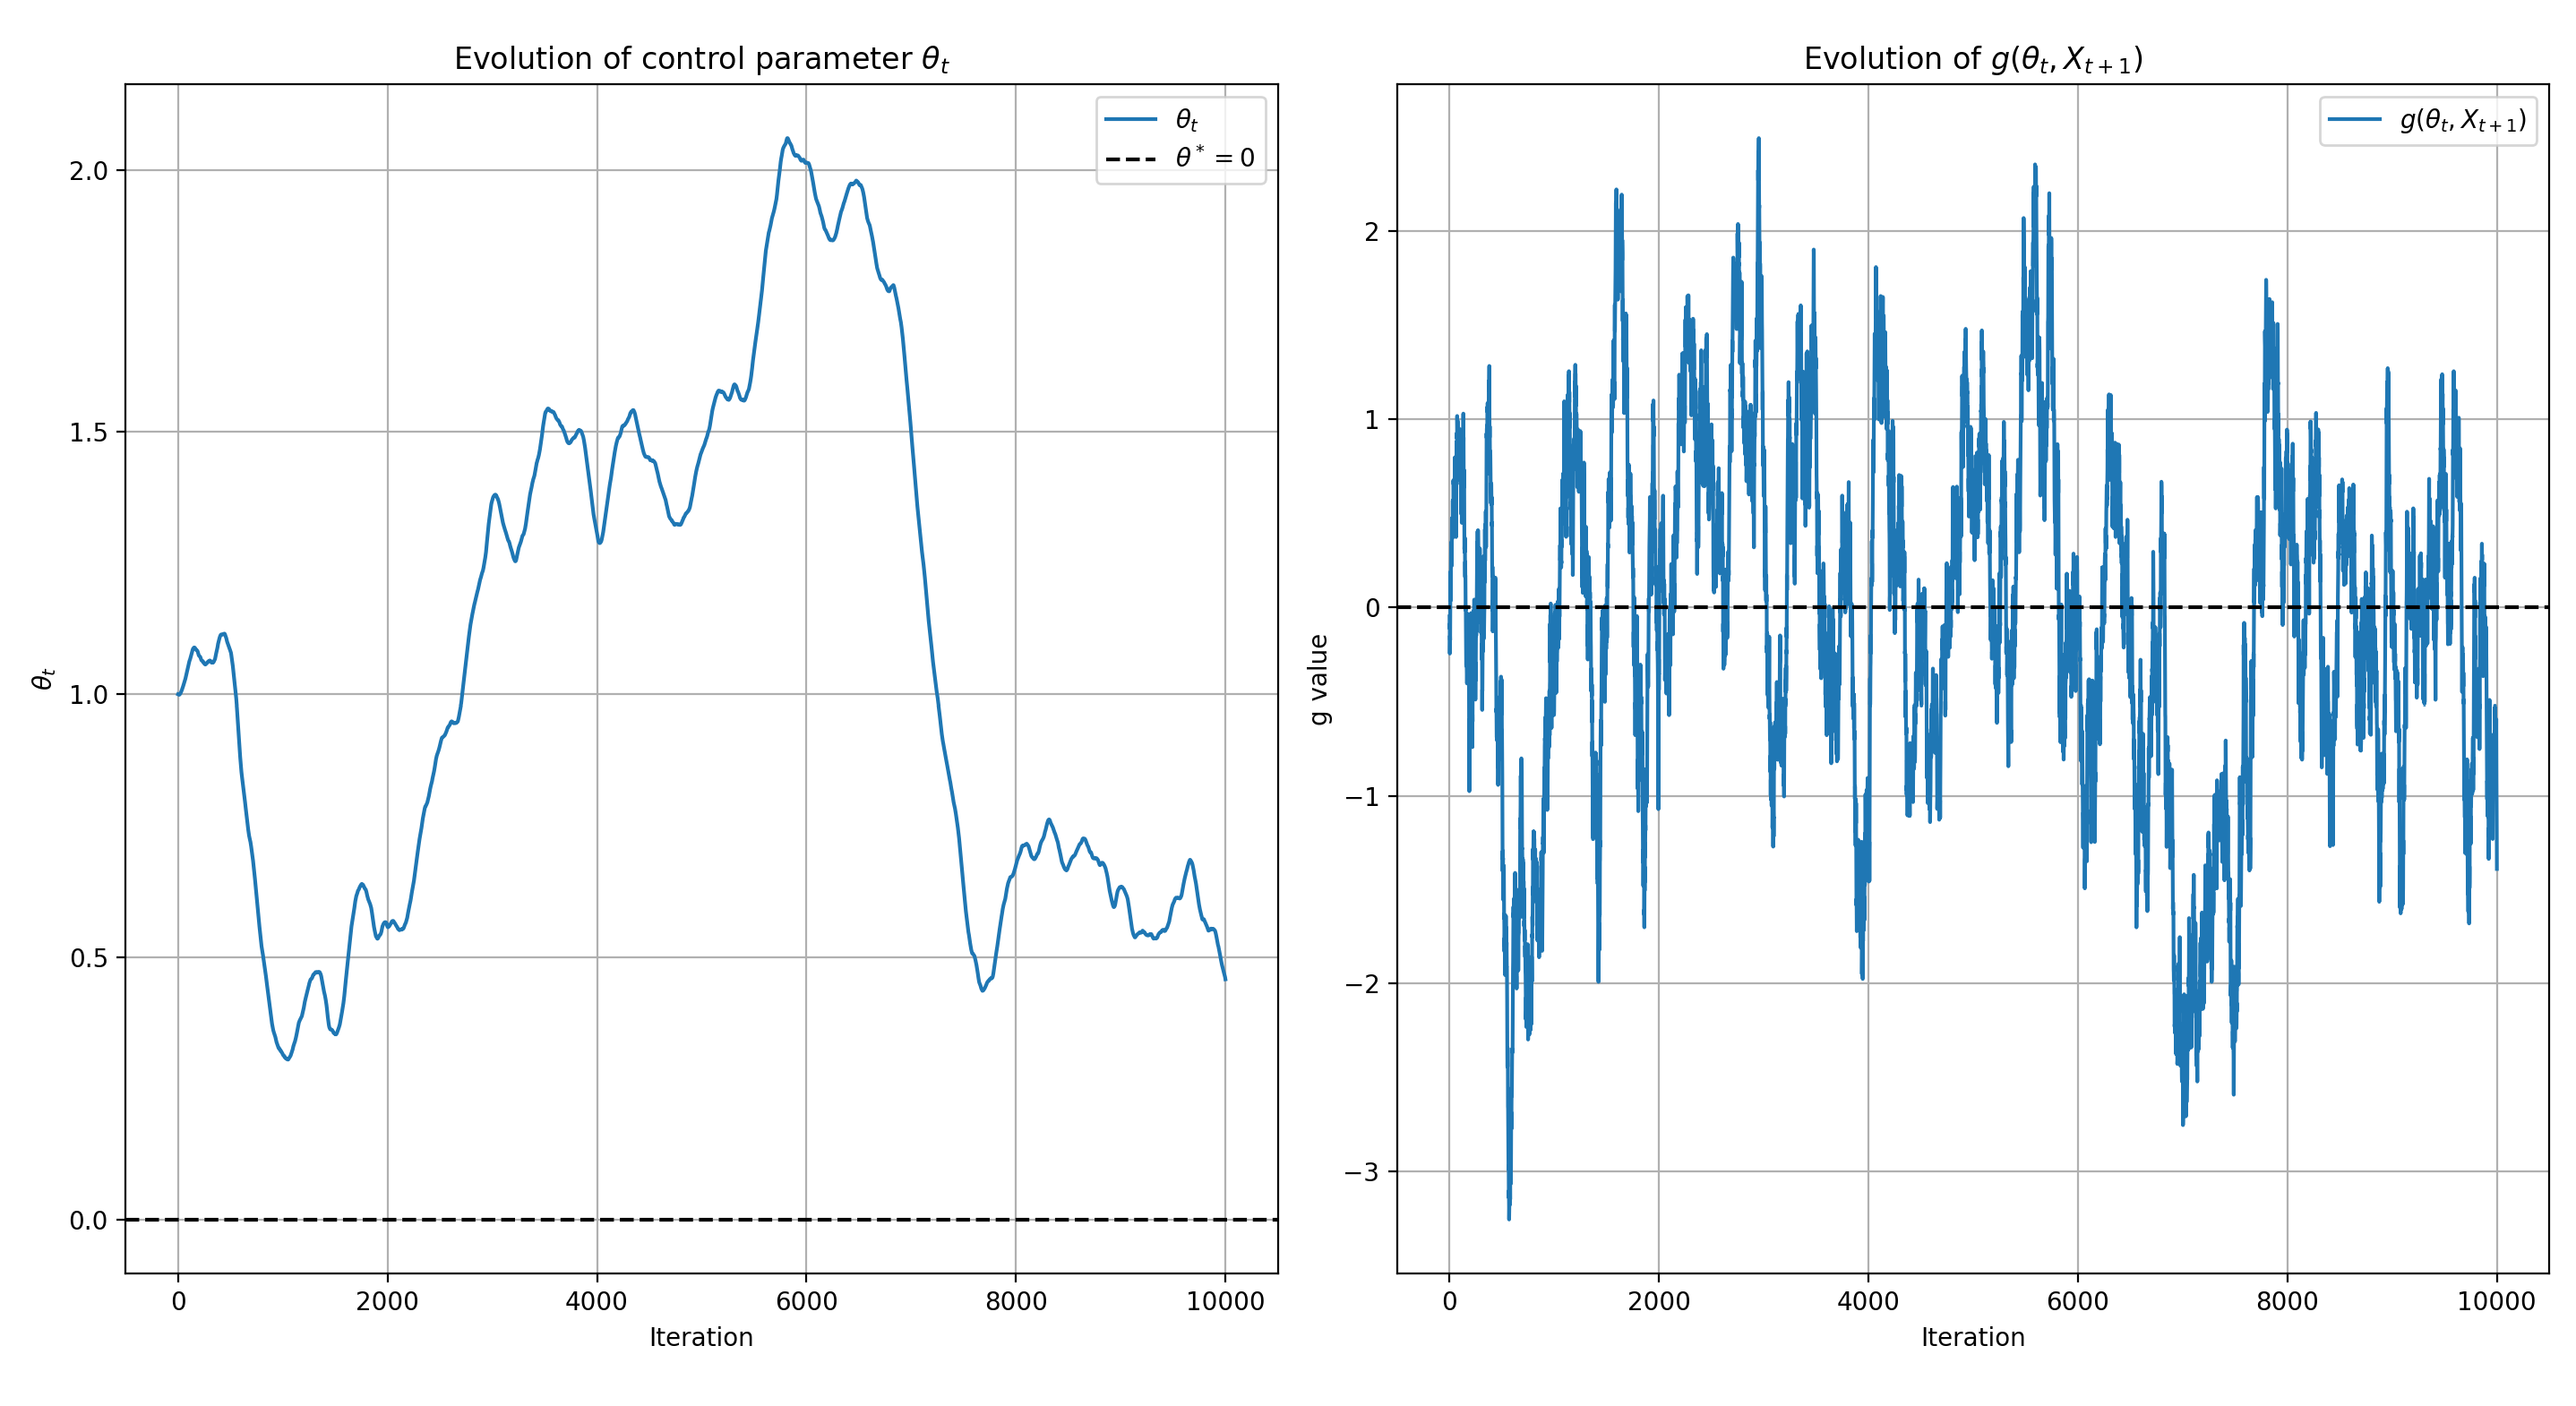
\includegraphics[scale=0.45]{fig1.png}
	 	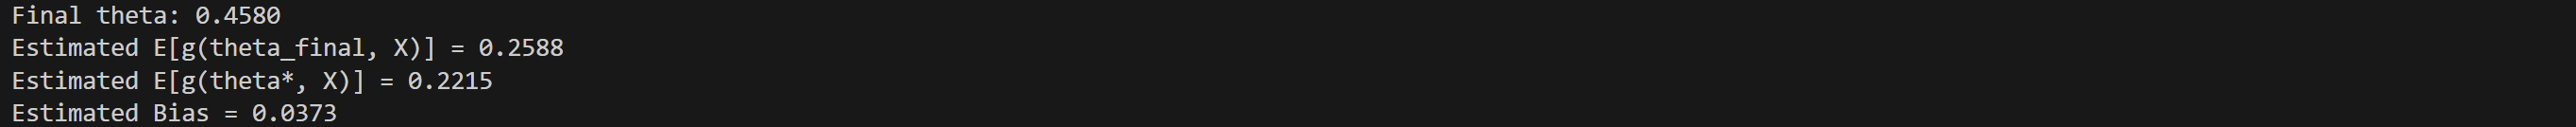
\includegraphics[scale=0.5]{fig2.png}
	 \end{center}
	 
	 \subsection*{Conclusion}
	 
	 This simulation tracks the evolution of the control parameter \(\theta_t\), the evaluated update function \(g(\theta_t, X_{t+1})\), and the bias over time. The algorithm converges toward the optimal value \(\theta^* = 0\), and the empirical bias decreases as expected, supporting both theoretical intuition and the Poisson equation structure.
	 
	 
	\bibliographystyle{ieee}
	\bibliography{ref.bib}
	
\end{document}